% There are two otion that can be provided to the uofathesis class
% 1) published - adjusts the declaration to include a statement regarding published materials. This is required if any chapters in your thesis have been published.
% 2) international - include this if you are an international student to exclude the paragraph regarding the Australian Government Research Training Program Scholarship 
\documentclass[published]{uofathesis}

% Any packages should go here
\usepackage{lineno,setspace}
\usepackage{caption}
\usepackage{booktabs}
\usepackage{amsmath,amssymb,amsfonts,amsbsy}
\usepackage{rotating,array,multirow}
\usepackage{textcomp}
\usepackage{afterpage, emptypage}
\usepackage{pdflscape}
\usepackage{graphicx,natbib} 
\usepackage{hyperref}
\usepackage{geometry}
\usepackage{layouts}
\usepackage{pdfpages}
\usepackage{epigraph} 
\DeclareMathOperator{\sech}{sech}

% SET MARGINS
\geometry{outer=20mm,inner=35mm}

% ADD HYPERLINKS TO DOCUMENT BUT MAINTAIN BLACK FONT
\hypersetup{colorlinks=true,allcolors=}

\title{An Off-lattice Computational Model for the Growth of Saccharomyces Cerevisiae}
\titlesize{\huge} % recommend using any of \large, \Large, \LARGE, \huge, \HUGE, depening on length of title. 
\author{Isaac Nakone}
\degree{Bachelor of Mathematical Sciences - Honours}
\department{Department of Mathematical Sciences}
\school{School of Computer and Mathematical Sciences}

% PATHS TO FIGURES - add these as needed
\graphicspath{
    {chapter1/figures/}
    {chapter2/figures/}
    }

% Use the includeonly command to work on individual chapters at a time.
% Comment out this command to build the entire document.
% \includeonly{chapter1/body}

\begin{document}
\frontmatter
\maketitle

% Create the following tables
\tableofcontents
\listoftables
\listoffigures

% HDR Declaration
\makedeclaration

% Import the various things
\chapter{Acknowledgements}

\textit{Where to begin?}
\\
Thank you to my supervisers, Ed Green and Sanjeeva Balasuriya,
for your enduring support during these \textit{two and a half} 
years.
\\
Thankyou to my highschool English teacher, Tanja, for teaching
me how to use form and technique in my writing.
\\
Thank you to my parents, Debbie and Alex, and to my sister,
Amelia. In your own way, you each provided the soil 
from which this thesis grew.
\\
Thank you to my literary friend, John, whose cerebral writing 
will have inspired a generation of \textit{rebels with a cause} by 
next Tuesday, I'm sure of it.
\\
Thank you to Kai and my other colleagues at \textit{Adelaide University}
for providing the environmental stresses to keep me growing. Ki 
was always willing to speak with me and offer his time. 
I am grateful.
\\
There appears to be a collection of \textit{Alex}'s in my life.
I thank you all dearly in one foul sweep. 
\\
To \textit{Radee}, for reminding be how to thinking critically 
and creatively at the same time.
\\
To Harry and Zehao and the other engineers one of whom is another \textit{Alex},
I appreciate you.
\\
To Giuseppe, thank you for introducing me to the \textit{bible of statistical mechanics}.
\\
For the fruitful \textit{Kong-Tchorbadjiev-Nakone} (KTN) correspondence,
for your years of philosphical musing.
\\
Thank you to \textit{cafe} staff at the university for your 
unassuming presence among the day-to-day emergence of new forms.
\\
Thankyou to the late philosophy Professor Michael Sugrue,
whose lectures, both young and old, were stunning depictions
of the daring heart of philosophy.
\\
Thankyou to \textit{ChatGPT},
for helping me externalise my interior geometry.
It materialised in the form of the great parable of baker's yeast.
\\
If there was anyone I forgot, I hope you are not offended.
\\

\textit{Isaac}

\chapter{Abstract}
Baker's yeast (\textit{Saccharomyces cerevisiae}) is capable 
of undergoing a pseudohyphal transition to filamentous growth in nutrient poor environments.
An algebraic representation of \textit{S. cerevisiae} cells is adapted from
computer graphics to model cellular division (mitosis) at low computational cost.
By reimagining mitosis as topological bifurcation using level sections 
of signed distance functions (SDFs) underpinned by a discrete mechanistic network, 
novel predictions about 
\textit{S. cerevisiae} colony morphology are made. Coupling 
the algbraic biomass field to a traditional reaction diffusion system 
for nutrient allows the relationship between metabolism 
and growth rate to be estimated for this agent based 
model (ABM). A measure for filamentous branching called compactness 
is introduced and related to cellular mobility under chemotaxis through
numerical experiments.  


\mainmatter
\introduction

\section{Kingdom Fungi}

Microfossils discovered in the Grassy Bay Formation 
(Shaler Supergroup, Artic Canada) dating back to the Proterozoic Eon, $2500$ to $538.8$ million years ago, were 
found to have fungal affinity (\cite{loron2019early}). Curiously, it took until 1969 for Fungi to be 
recognised in plant ecologist Robert Whittaker's work as part of a taxonomic kingdom, Kingdom Fungi,
which is distinct from Kingdom Plantae (\cite{whittaker1969new}). Today, locating fungal species 
in phylogenetic lineages is facilitated through colonial morphology imaging as a first 
estimate. More advanced experimental techniques such as transmission 
electron microscopy (TEM) can provide  
conclusive identification (\cite{loron2019early}) of fungal samples.
\\

Nonetheless, morphological features observed in fungal strains such as fission yeast 
(\textit{Schizosaccharomyces pombe}) are sometimes cited as the reason 
why yeast is broadly considered a ``model organism'' (\cite{hayles2018introduction}).
Cell Biologist Murdoch Mitchison was able to study the fission yeast cell cycle in 1957 for instance,
because the length of the rod shaped cells of \textit{S. pombe} reflected their stage in the cell cycle.
It happens to be an \textit{S. pombe} spore grown on malt extract agar that was imaged in exquisite detail via 
X-ray diffraction microscopy by \cite{jiang2010quantitative}. By 3D 
reconstruction techniques \cite{jiang2010quantitative} visualised the organelles
present in the unstained (and unsectioned) spore at a resolution of $50-60 \ nm$ 
producing isosurfaces of cellular organelles such as the endoplasmic reticulum, 
vacuole and cell wall.
\\

Contemporary advancements in computer hardware facilitate 
the ability for big datasets such as 3D morphological data 
obtained from yeast to be analysed mathematically. \cite{clermont2015inverse} 
discuss the ``inverse problem" in mathematical biology, which is to determine a model 
from noisy, complex and extensive biological data whilst minimising bias. This often 
comes in the framework of model parameter estimation which 
can be accelerated using fairly systematic deep learning techniques. Still, the predictive power
of a mathematical model is always limited by the bias implicit (or explicit) in its assumptions.
\\

Biology is inherently multi-scale and the problem 
of bridging between scales is named the ``translational challenge'' (\cite{an2009agent}).
The interplay between the phenotypical properties of a filamentous yeast colony and 
its genotype, is one such challenge. Indeed, the eukaryote \textit{S. pombe}, has a similar 
cytoskeletal organisation to a human tissue cell as well as analogous DNA transcription mechanisms 
(\cite{hoffman2015ancient}) and yet human tissue 
morphology vastly differs from fission yeast.
\\

\cite{an2009agent} position agent-based models (ABMs), dating back to cellular automata, as well suited to the 
 translational challenge for a number of reasons. These include the ability 
 for ABMs to model morphological emergence from simple and modular rules. These rules 
 are constructed from a qualitative understanding of the underlying mechanisms of for instance 
 \textit{S. pombe} intracellular stresses which could be based on some basic assumptions
 about cellular elasticity. Importantly, ABMs are easy to deploy acting 
 as a cheap alternative to \textit{in vitro} experiments with fungal species.
 \\

 Multi-cellular agent based modelling of \textit{S. pombe} or baker's yeast 
 (\textit{Saccharomyces cerevisiae}) is of interest to number of scientific  
 communities. On the one hand, due to the molecular similarity of yeast to human 
 cells it can serve as a model organism that can ethically be grown, and on 
 the other it is of intrinsic interest to philogeneticists who study the origin 
 of life on Earth. Morphological studies using ABMs can also provide breweries and 
 food processing industries with practically useful findings to 
 set up ideal growth conditions for cultures prior to expensive 
 industrial implemenatations. Indeed \textit{pombe} is Swahili 
 for ``booze'', being originally observed in contaminated 
 millet beer delayed on route from East Africa to Germany (\cite{hayles2018introduction}).
 \\

 In this work, a dynamic off-lattice agent based modelling framework for \textit{S. cerevisiae} colonial morphology 
 is proposed and implemented. As opposed to fission yeast, \textit{S. cerevisiae} exhibits 
 budding and can be induced into a filamentous regime called pseudohyphal growth
 in which cells become elongated leading to overall branching patterns 
 in the colonial morphology. The off-lattice ABM developed in \cite{li2024off} 
 inspired the modelling of the pseudohyphal \textit{S. cerevisiae} regime 
 presented here, though it uses a vastly different computational methodology.
 \\

 \cite{li2024off} use approximate bayesian computatation (ABC)
 to infer model parameters within the context of a probabilistic (and spatial) branching simulation, 
 yielding remarkable fits to micrographs of filamentous yeast. Building 
 from the experimental observations of pseudohyphal growth presented in 
 \cite{gimeno1992unipolar}, Li et al. dispense with diffusion limited growth (DLG) which is
shown by \cite{tronnolone2018diffusion} to only be a peripheral mechanism in filamentous 
colony shape.
\\

Whilst pseudohyphal growth dynamics
have proved to be the dominant growth mechanism (\cite{tronnolone2018diffusion}) for 
\textit{S. cerevisiae} in nutrient poor environments, it is the aim of the present 
work to reintroduce a diffusive nutrient medium in the hope of defining 
\textit{to what extent} these two phenomena intertwine.
\\

\cite{brown2021rigid} develop rigid body modelling for multi-cellular colonies using 
an ABM which represents each cell as a deformable polygon. The emphasis in the model 
of Brown et al. is to represent to process of cell division in diverse biological 
settings through the addition of new nodes and edges to each polygonal cell. 
In contrast, \cite{li2024off}, use static ellipsoidal cells that are added into the simulation
abruptly. \cite{li2024off} instead focus on the ability to fit their model 
to experimental micrographs of \textit{S. cerevisiae} using statistical methods.
In fact, this choice seems to reflect a gap in the multi-cellular modelling literature:
\textit{how can cell division be represented without the artificial inclusion of new parameters?}
\\

In both the work of \cite{van2020quantitative}, and the ABM of 
\cite{brown2021rigid}, the dynamics of the colony 
are derived from the dynamcis of individual cells which are represented
by meshes with time-dependent topology as well as geometry. However ingenious this idea may be, 
computation quickly becomes intractible for large colonies
due to the increasing size of the underlying system of ordinary differential equation (ODEs)
for the node states. Most serious ABMs need supercomputers, however
the computationally costly use of meshed cells is circumvented in the current work by employing 
an algebraic representation of cell geometry.
\\





In Keener and Sneyd's foundational textbook on cellular physiology 
(\cite{keener2009mathematical}), the law of mass action is 
introduced as the fundamental law of chemical reactions, 
the process of transformation comprises the living cell. The law of mass 
action states that for the reaction 
\begin{equation*}
    A + B \xrightarrow{k} C,
\end{equation*}
in which chemicals $A$, $B$ react to form the product $C$, the rate of change of the concentration of $C$, 
call it $c$ (in mol$\cdot L^{-1}$) is proportional to the product of the concentration 
of $A$ and $B$, given by $a$ and $b$, respectively. Sequences of interrelated chemical 
reactions induce systems of first order non-linear ordinary differential equations 
(ODEs). These are called a chemical reaction network.
\\

It is suprising then that much of the cell's functionality and behaviour 
can, in theory, be derived from these chemical reaction networks, however
we would not expect all behaviour to be derivable from this model alone.
This is for two reasons,

The art of mathematical biology is to capture a biological phenomenon with the 
simplest model possible. Another concern which appears in the connection between 
applied and pure mathematics, is that of ensuring the model that one selects is 
amenable to rigorous analysis. This further reinforces the requirement that the 
model be as simple as possible, but no simpler. Indeed, a model that is sufficiently 
crystallized so as to capture the essential details of a physical effect, will 
necessarily not capture everything observable, but has more chance to be useful, 
since it directs our thinking away from extraneous features.
\\
\\
What is essential in the study of biological systems? One essential aspect is the 
phenomenon of growth. Growth, when seen on its own, without reference to biology, 
is simply ``change over time". The standard tool for this is calculus, which in its 
more developed form, is called differential geometry. A cell colony will be modelled 
here as a subset of $\mathbb{R}^n$ where $n = 1,2,3$. In order for that set to 
``change over time", namely, for the cell to be parametrized by a real number 
$t \in \mathbb{R}_{\geq 0}$, the geometry of the colony needs to be represented 
by a finite list of parameters. The most simple way to do this, which comprises 
one of the models developed here, is to represent each cell as a disk in 
$\mathbb{R}^2$ with radius $r = r(t) \in \mathbb{R}_{\geq 0}$ centered at 
the position $(x(t),y(t)) \in \mathbb{R}^2$. The advantage to this approach 
is that it is more computationally efficient as compared to models which 
represent each cell as a deformable polygon, for instance.
\\
\\
The question remains: how can cell division be achieved within mathematical 
growth models? It does not seem obvious except via the continual addition of 
new parameters, such as new cell radii and positions. As we will see, taking 
seriously the question of mitosis from a topological standpoint will yield a 
generalized model for systems in which geometric changes and topological changes 
can be captured simultaneously. Why is the topology important in the case of biological growth? 
\\
\\
As a motivating example, consider the graph of the function $f(x) = x^2$. 
Now consider the time-dependent set given by $C(t) = f^{-1} (\{t\})$ where 
$t \in \mathbb{R}_{\geq 0}$ is a time parameter. When $t=0$, $C(0) = \{ 0\}$ 
(only one element), but when $t=1$, $C(1) = \{ -1, +1  \}$, which has two elements, 
and, likewise for $t=2$ where $C(t) = \{ -\sqrt{2}, +\sqrt{2}  \}$. This example 
shows that a catastrophic change (a bifurcation) can occur in $C(t)$ during a smooth 
change in $t$. A subtle modification to this model is to consider $f_t(x) = x^2-t$ 
and fix $C(t) = f^{-1}_t(\{0 \})$. That is, instead of sliding up the query point $t$, 
we slide down the whole smooth manifold given by $(x,f_t(x))$ such that $x \in \mathbb{R}$. 
The set $C(t)$ is actually called a level-$0$ set. We will just call this a level set of $f_t$.
\\
\\
We can consider level sets of functions from $\mathbb{R}^n$ to $\mathbb{R}$ for $n = 2,3$ 
as well. In these cases, the level sets are, respectively, level curves and level surfaces. 
A analogous example for $n=2$, is the set of functions $f_t(x,y) = x^2+y^2-t$, the level 
curves of which look like circles centered at the origin of radius $\sqrt{t}$.
\\
\\
This level of generalization will not be sufficient for our purposes, since the 
type of manifolds that we will be dealing with will not in general be representable 
as graphs of functions. To see this, consider the fact that a vertical line in the 
$xt$-plane is a perfectly reasonable representation of a stationary cell, and yet 
there's no function (of $x$) that has a vertical line graph. What is required is 
that $C(t) = \{ p \in M_t \ | \ \textrm{the last component of $p$ is $0$} \}$ where 
$M_t$ is a time dependent smooth manifold. The requirement that $M_t$ is smooth for 
all $t$ is imposed so that the theory of smooth manifolds can be brought to bear on 
the problem. What we will consider are smooth manifolds $M_t \subset \mathbb{R}^{n+1}$ 
where $n$ is the dimension in which the colony exists. For instance, a two-dimensional 
colony would be represented by
\begin{equation}
        C(t) = \{ p \in M_t \subset \mathbb{R}^3 \ | \ p_3 = 0  \}.
\end{equation}
A three-dimensional colony would be represented by
\begin{equation}
        C(t) = \{ p \in M_t \subset \mathbb{R}^4 \ | \ p_4 = 0  \}.
\end{equation}
\\
\\
In the subdiscipline of abstract algebra called ring theory, it is typical to 
consider the polynomial ring over the real field in two variables $\mathbb{R}[x,y]$ 
wherein the typical element looks like
\begin{equation}
    p(x,y) = \sum_{n,m} a_{nm} x^n y^m,
\end{equation}
where $n,m$ are non-negative integers, and $a_{nm}$ is a real coefficient.
The set $\mathbb{R}[x,y]$ is closed under multiplication and addition because 
polynomial multiplication and addition yields another real polynomial. In this 
thesis, a cell will be modeled as a level set of the quartic given by
\begin{equation}
    f(x,y) = ax^4 +bx^3+cx^2 +dx +e+
\end{equation}


At the beginning, we imagine a colony of yeast cells that is restricted to move 
along a straight line. The colony is therefore modeled as a set of real numbers 
$C \subset \mathbb{R}$. Like an archipelago of small islands, the colony as a whole 
is composed of closed sets, $C_j$ where $j \in \mathbb{N}$ indexes over the cells. 
Therefore, the colony is a disjoint union of these individual cells,
\begin{equation*}
    C = \coprod_{j=1}^N C_j
\end{equation*}
and $N$ is the total cell count. Closed sets (in the standard topology on 
$\mathbb{R}$) are chosen to represent the cells for the technical reason that 
a point (singleton) may also constitute a cell. In fact, we further restrict 
each cell to a closed interval $C_j = [a_j, b_j]$.
\\
\\
As we shall see in general, all we require is that each cell have no holes. 
Another way of saying this is that each cell is homeomorphic to a singleton 
(which works in $\mathbb{R}^2$ and $\mathbb{R}^3$ as well). Finally, the closed 
interval $[a_j,b_j]$ will be called a parametrization of the cell $C_j$: this is 
important to note for the generalization to $\mathbb{R}^2$ and $\mathbb{R}^3$, 
where parametrizations must also be constructed.
\\
\\
The mechanism of mitosis must account for the fact that several cells can 
undergo fission at the same time, or more aptly, they undergo mitosis independently. 
The most general formulation, which is also simple to implement computationally is the 
addition of a non-intersecting singleton $\{x  \}$ to the set $C$. Note, that this 
mechanism is chosen principally for the fact that it conserves the Lebesgue measure of the colony,
\begin{equation*}
    l(C \cup \{x\} ) = l(C),
\end{equation*}
where $C \cup \{x\} $ is the colony after mitosis has occurred, since singletons have measure $0$. 
\\
\\
Of course, some restrictions must be applied to the choice of 
$x \in \mathbb{R} \setminus C$. Since, we are always working in 
Euclidean spaces (for practical scenarios), we may as well require that 
$x$ is close to $C$ in the sense that for all $c \in C$ we have that 
$d(c,x) < \delta$ for some small positive amount $\delta$ where 
$d: \mathbb{R} \times \mathbb{R} \rightarrow \mathbb{R}_{\geq 0}$ 
is the Euclidean metric on $\mathbb{R}$ (which is easily generalized to 
higher dimensions). This parameter $\delta$ represents how the colony spreads out.
\\
\\
A profitable aspect of this model for cell colonies is that it unifies 
the topological aspects of the colony (it is always homeomorphic to a finite 
set of points or the empty set), and the measure theoretic properties (one can 
speak of getting more cells without changing the total measure). This means we 
can separate the dynamics of cell division from the dynamics of the geometric 
growth of the cells, i.e. the change in $a_j$ and $b_j$. One simple way to do 
this is to supply an ordinary differential equation for the measure of the 
colony $V = l(C)$, and equip this with a discrete time update equation for number of cells. 
\\
\\
To move us closer to a manageable computer implementation of cell colony growth, 
we consider the simple growth model given by,
\begin{equation*}
    \frac{dV(t)}{dt} = g(t),
\end{equation*}
\begin{equation*}
    N_{n+1} = 2N_n,
\end{equation*}
where $g(t)$ is a growth function. Now we need apply some equation for 
how each cell grows. For sake of simplicity, say that for all cells $j$, the cell measure $V_j$ grows as
\begin{equation*}
    \frac{dV_j(t)}{dt} = g_j(t), \ \ t \geq m_j,
\end{equation*}
 where $g_j(t)$ is a cellular growth function such that 
 $V_j(t) \rightarrow V_f$ is the final cellular volume, and $m_j$ is the 
 birth time of the cell. This actually is not enough to specify the whole 
 colony geometry. So how do we pin down the geometry?
\\
\\
The geometry and how its dynamics evolve of course depends on the 
chosen parametrization of each cell. For our purposes, we will 
consider $C_j = \bar{B} (x_j, \varepsilon_j)$ where
\begin{equation*}
    \bar{B} (x_j, \varepsilon_j) = \{ x \in \mathbb{R} : d(x_j,x) \leq \varepsilon_j \},
\end{equation*} 
which is called the closed ball centered on $x_j$ of radius $\varepsilon_j$.
 That means $a_j = x_j-\varepsilon_j$, and $b_j = x_j+\varepsilon_j$. It is 
 more convenient to use this parametrization since closed balls are defined 
 in higher dimensions as well. Another important benefit to the closed ball 
 is that whenever $\varepsilon_j = 0$, $\bar{B} (x_j, 0) = \{ x_j\}$. Also, 
 the volume of each cell is simply $V_j = 2\varepsilon_j$ which tells us that
  the volume is completely independent of the cell center position $x_j$.
\\
\\
Now we easily obtain a nice formula for $\varepsilon_j(t)$  defined for $t \geq m_j$ as
\begin{equation*}
    \varepsilon_j(t) = \frac{1}{2} \int_{m_j}^t g_j(s)ds.
\end{equation*}
But, recall, since the $C_j$ are each disjoint, $V$ is given by
\begin{equation*}
    V = l(C) = \sum_{j=1}^N l(C_j) = \sum_{j=1}^N V_j.
\end{equation*}
This applies to the time derivative too, yielding 
\begin{equation*}
    \frac{dV(t)}{dt} = \sum_{j=1}^N \frac{dV_j(t)}{dt}.
\end{equation*}
This means that the colony and cell growth functions must be related by the following,
\begin{equation*}
    g(t) = \sum_{j=1}^N g_j (t).
\end{equation*}
Our functions $g_j(t)$ were defined for $t \in [m_j, +\infty)$ which means they have
 different domains. To make the analysis easier, we build these functions by taking
  linear combinations of basis hat functions (defined for $t \in [0, +\infty)$). 
  The basis functions have compact support and are given piecewise by,
\begin{equation*}
    \varphi_i(t) = \begin{cases} 
      \frac{t-t_{i-1}}{h}, & t \in [t_{i-1}, t_i] \\
      \frac{t_{i+1}-t}{h}, & t \in [t_{i}, t_{i+1}] \\
      0, & \textrm{otherwise}, 
   \end{cases}
\end{equation*}
where $h$ is the smallest time step, $t_0 = 0$ and $t_i = ih$ for $i \in \mathbb{N}$.
 Hence, each $g_j(t)$ can be extended to a definition on all of $\mathbb{R}_{\geq 0}$ by
\begin{equation*}
    \tilde{g}_j(t) = \sum_{i=1}^{\infty} g_j(t_i) \varphi_i(t) =\sum_{i=1}^{\infty} g_{ij} \varphi_i(t) .
\end{equation*}
Now that the $g_{ij}$ are defined on the same domain, we can further restrict to
 $i \leq T$ where $T$ is the total number of time steps. This means that the time 
 dependence is now fixed by a finite number of parameters, $g_{ij}$. Summing over
  $j$, we get that
\begin{equation*}
    \tilde{g}(t) = \sum_{j=1}^N \sum_{i=1}^{T} g_{ij} \varphi_i(t).
\end{equation*}
\chapter{Literature Review}

\section{Modelling Kingdom Fungi}

Microfossils discovered in the Grassy Bay Formation 
(Shaler Supergroup, Artic Canada) dating back to the Proterozoic Eon, $2500$ to $538.8$ million years ago, were 
found to have fungal affinity (\cite{loron2019early}). Curiously, it took until 1969 for Fungi to be 
recognised in plant ecologist Robert Whittaker's work as part of a taxonomic kingdom, Kingdom Fungi,
which is distinct from Kingdom Plantae (\cite{whittaker1969new}). Today, locating fungal species 
in phylogenetic lineages is facilitated through colonial morphology imaging as a first 
estimate. More advanced experimental techniques such as transmission 
electron microscopy (TEM) can provide  
conclusive identification (\cite{loron2019early}) of fungal samples.
\\

Nonetheless, morphological features observed in fungal strains such as fission yeast 
(\textit{Schizosaccharomyces pombe}) are sometimes cited as the reason 
why yeast is broadly considered a ``model organism'' (\cite{hayles2018introduction}).
Cell Biologist Murdoch Mitchison was able to study the fission yeast cell cycle in 1957 for instance,
because the length of the rod shaped cells of \textit{S. pombe} reflected their stage in the cell cycle.
It happens to be an \textit{S. pombe} spore grown on malt extract agar that was imaged in exquisite detail via 
X-ray diffraction microscopy by \cite{jiang2010quantitative}. By 3D 
reconstruction techniques \cite{jiang2010quantitative} visualised the organelles
present in the unstained (and unsectioned) spore at a resolution of $50-60 \ nm$ 
producing isosurfaces of cellular organelles such as the endoplasmic reticulum, 
vacuole and cell wall.
\\

Contemporary advancements in computer hardware facilitate 
the ability for big datasets such as 3D morphological data 
obtained from yeast to be analysed mathematically. \cite{clermont2015inverse} 
discuss the ``inverse problem" in mathematical biology, which is to determine a model 
from noisy, complex and extensive biological data whilst minimising bias. This often 
comes in the framework of model parameter estimation which 
can be accelerated using fairly systematic deep learning techniques. Still, the predictive power
of a mathematical model is always limited by the bias implicit (or explicit) in its assumptions.
\\

Biology is inherently multi-scale and the problem 
of bridging between scales is named the ``translational challenge'' (\cite{an2009agent}).
The interplay between the phenotypical properties of a filamentous yeast colony and 
its genotype, is one such challenge. Indeed, the eukaryote \textit{S. pombe}, has a similar 
cytoskeletal organisation to a human tissue cell as well as analogous DNA transcription mechanisms 
(\cite{hoffman2015ancient}) and yet human tissue 
morphology vastly differs from fission yeast.
\\

\cite{an2009agent} position agent-based models (ABMs), dating back to cellular automata, as well suited to the 
 translational challenge for a number of reasons. These include the ability 
 for ABMs to model morphological emergence from simple and modular rules. These rules 
 are constructed from a qualitative understanding of the underlying mechanisms of for instance 
 \textit{S. pombe} intracellular stresses which could be based on some basic assumptions
 about cellular elasticity. Importantly, ABMs are easy to deploy acting 
 as a cheap alternative to \textit{in vitro} experiments with fungal species.
 \\

 Multi-cellular agent based modelling of \textit{S. pombe} or baker's yeast 
 (\textit{Saccharomyces cerevisiae}) is of interest to number of scientific  
 communities. On the one hand, due to the molecular similarity of yeast to human 
 cells it can serve as a model organism that can ethically be grown, and on 
 the other it is of intrinsic interest to philogeneticists who study the origin 
 of life on Earth. Morphological studies using ABMs can also provide breweries and 
 food processing industries with practically useful findings to 
 set up ideal growth conditions for cultures prior to expensive 
 industrial implemenatations. Indeed \textit{pombe} is Swahili 
 for ``booze'', being originally observed in contaminated 
 millet beer delayed on route from East Africa to Germany (\cite{hayles2018introduction}).
 \\

 \section{Agent based modelling in context}

 In the current thesis, a dynamic off-lattice agent based modelling framework for \textit{S. cerevisiae} 
 colonial morphology 
 is proposed and implemented. As opposed to fission yeast, \textit{S. cerevisiae} exhibits 
 budding and can be induced into a filamentous regime called pseudohyphal growth
 in which cells become elongated leading to overall branching patterns 
 in the colonial morphology. The off-lattice ABM developed in \cite{li2024off} 
 inspired the modelling of the pseudohyphal \textit{S. cerevisiae} regime 
 presented here, though it uses a vastly different computational methodology.
 \\

 \cite{li2024off} use approximate bayesian computatation (ABC)
 to infer model parameters within the context of a probabilistic (and spatial) branching simulation, 
 yielding remarkable fits to micrographs of filamentous yeast. Building 
 from the experimental observations of pseudohyphal growth presented in 
 \cite{gimeno1992unipolar}, Li et al. dispense with diffusion limited growth (DLG) which is
shown by \cite{tronnolone2018diffusion} to only be a peripheral mechanism in filamentous 
colony shape.
\\

Whilst pseudohyphal growth dynamics
have proved to be the dominant growth mechanism (\cite{tronnolone2018diffusion}) for 
\textit{S. cerevisiae} in nutrient poor environments, it is the aim of the present 
work to reintroduce a diffusive nutrient medium in the hope of defining 
\textit{to what extent} these two phenomena intertwine.
\\

\cite{brown2021rigid} develop rigid body modelling for multi-cellular colonies using 
an ABM which represents each cell as a deformable polygon. The emphasis in the model 
of Brown et al. is to represent to process of cell division in diverse biological 
settings through the addition of new nodes and edges to each polygonal cell. 
In contrast, \cite{li2024off}, use static ellipsoidal cells that are added into the simulation
abruptly. \cite{li2024off} instead focus on the ability to fit their model 
to experimental micrographs of \textit{S. cerevisiae} using statistical methods.
In fact, this choice seems to reflect a gap in the multi-cellular modelling literature:
\textit{how can cell division be represented without the artificial inclusion of new parameters?}
\\

In both the work of \cite{van2020quantitative}, and the ABM of 
\cite{brown2021rigid}, the dynamics of the colony 
are derived from the dynamcis of individual cells which are represented
by meshes with time-dependent topology as well as geometry. However ingenious this idea may be, 
computation quickly becomes intractible for large colonies
due to the increasing size of the underlying system of ordinary differential equation (ODEs)
for the node states. Most ABMs need supercomputers, however
the computationally costly use of meshed cells is circumvented in the current work by employing 
an algebraic representation of cell geometry.
\\

\section{From algorithmic botany \\ 
         to algorithmic mycology}

The model defined in Chapter 2 of this thesis is underpinned by a ``growing network" which is an example 
of a graph-rewriting system. The natural precursor 
to this concept is the mathematical corpus of biologist Aristid Lindenmayer, whose work 
on cellular interactions in plants and fungi based on \textit{sequential machines}, 
\cite{lindenmayer1968mathematical}, developed 
into the notion of an $L$-system, \cite{prusinkiewicz2012algorithmic}. An $L$-system
is a string-rewriting system that applies a conversion rule to each letter in a word 
simultaneously, \cite{prusinkiewicz2012algorithmic}. For example,
the rules (or ``productions'') that sends $A \rightarrow AB$ and $B \rightarrow A$,
would evolve the input word, $A$, as follows,
\begin{equation*}
\begin{split}
&A \\
&AB \\
&ABA \\
&ABAAB \\
&ABAABABA, \\
\end{split}
\end{equation*}
\\
which could continue on indefinitely. Taken together,
the alphabet, $\{A, B\}$, the productions, $\{ A \rightarrow AB, B \rightarrow A \}$, and 
the intial word, $A$, comprise an $L$-system. 
\\

The ideas  
of Lindenmayer have been taken up by the Algorthmic Botany Group \cite{algorithmicbotany_papers}
led by Przemyslaw Prusinkiewicz whose website has links to the group's papers dating
back to the 1980s. In a recent paper from 2024, Coen and Prusinkiewicz study 
two modes of developmental timing mechanisms in plants, one of them being related 
to instrinsic molecular processes and one of them being growth-dependent, for instance, dependent 
on space being available \cite{coen2024developmental}. Their computational methology,
which is of relevance to the current thesis, seems to be based on novel $L$-system
softwares developed in the Algorithmic Botany Group. Even by the year 2012, 
Boudon et al. \cite{boudon2012py} published \textit{L-Py}, a Python package 
for modelling plant architecture based on a dynamic language.  
\\

The key innovation of the present thesis work is to 
bring into contact three distinct areas of 
study into one interdependent framework for studying mycology. These three 
areas are,
\begin{itemize}
    \item Graph rewriting as exemplified in botanical $L$-system work,
    \item Constructive solid geometry (CSG) in computer vision,
    \item Reaction-diffusion partial differential equations (PDEs),
          as studied in mathematical biology \cite{turing1990chemical}.
\end{itemize}
The first and third of these areas have already been introduced in the work of 
the algorithmic botany group and recent work from \cite{tronnolone2018diffusion}.

\section{Implicit surfaces and constructive solid geometry (CSG)}

The three most commom ways 
of representing a 2D or 3D object mathematically are parametric, polygonal,
or implicit techniques. For instance, a parametric representation of the 
points of a circle is $(\cos{t}, \sin{t})$ where $t$
is a real number. Alternatively, a polygonal representation of a circle
would be a regular $n$-gon which could be made a better approximation 
as $n \rightarrow \infty$. This sort of approach is effectively used 
by \cite{van2020quantitative} and \cite{brown2021rigid} in their solid mechanics
frameworks. Mesh based modelling has the advantage of locality in that 
deformations to the shape can be made by moving a node in the mesh
without changing it globally which gives more flexibility.
A limitation which has already been mentioned is that mesh based models, 
particualary in the context of growth, quickly lead to huge node numbers 
which imply supercomputers as a necessity for large colony simulations.
\\

Conversely, implicit representations of smooth geometric shapes are defined 
globally at the cost of local specificity. In three dimensions, one can 
define the surface of a sphere as set of points in $\mathbb{R}^3$ 
which satisfy the following equation,
\begin{equation*}
    x^2 + y^2 + z^2 - 1 = 0.
\end{equation*}
This is a special case of what is known as a quadric surface,
which is defined as the set of points which satisfy $f(x,y,z) =0$, where
\begin{equation*}
\begin{split}
    f(x,y,z) = p_1 x^2 + p_2 xy + p_3 xz + p_4 x + p_5 y^2 + p_6 yz + p_7 y + p_8 z^2 + p_9 z + p_{10},
\end{split}
\end{equation*}
as introduced in \cite{blinn1982generalization}. The full generalisation to the notion 
of implicit curves would require a precise notion of what space 
the functions, $f$, belong to. In the case of quadric surfaces, 
the functions belong to the ring of polynomials in $x$, $y$ and $z$, written as 
$\mathbb{R}[x,y,z]$, but more exotic settings can be used.
\\

In many contexts where specificity and local shape control are essential, 
implicit curves are not the best tool. Consider the quadric surface defined above.
The only way to modify the surface is to tune the parameters $p_1, ..., p_{10}$ but 
doing this results in a change to the whole surface which requires 
advanced mathematical machinery to control. This is where constructive solid geometry (CSG) comes 
in. 
\\

CSG is a technique used to build new implictely represented shapes from old ones.
In multi-cellular modelling, where the individual cell geometry 
is relatively fixed but there 
are regular topological bifurcations corresponding to cell division,
CSG is ideal and suprising has not been implementated in mycology agent 
based models as far as the author is aware. The graphical technique used 
in the current thesis is analogous to ``Metaballs'' or ``Blobby modelling'' which is 
implemented in C++ by \cite{kommareddy20143d}. The individual balls, 
modelled by quadric surfaces $f_1$ and $f_2$, are blended together 
into a new quadric surface $f(x,y,z) = f_1(x,y,z) + f_1(x,y,z)$.
\\



In Keener and Sneyd's foundational textbook on cellular physiology 
(\cite{keener2009mathematical}), the law of mass action is 
introduced as the fundamental law of chemical reactions, 
the process of transformation comprises the living cell. The law of mass 
action states that for the reaction 
\begin{equation*}
    A + B \xrightarrow{k} C,
\end{equation*}
in which chemicals $A$, $B$ react to form the product $C$, the rate of change of the concentration of $C$, 
call it $c$ (in mol$\cdot L^{-1}$) is proportional to the product of the concentration 
of $A$ and $B$, given by $a$ and $b$, respectively. Sequences of interrelated chemical 
reactions induce systems of first order non-linear ordinary differential equations 
(ODEs). These are called a chemical reaction network.
\\

It is suprising then that much of the cell's functionality and behaviour 
can, in theory, be derived from these chemical reaction networks, however
we would not expect all behaviour to be derivable from this model alone.
This is for two reasons,

The art of mathematical biology is to capture a biological phenomenon with the 
simplest model possible. Another concern which appears in the connection between 
applied and pure mathematics, is that of ensuring the model that one selects is 
amenable to rigorous analysis. This further reinforces the requirement that the 
model be as simple as possible, but no simpler. Indeed, a model that is sufficiently 
crystallized so as to capture the essential details of a physical effect, will 
necessarily not capture everything observable, but has more chance to be useful, 
since it directs our thinking away from extraneous features.
\\
\\
What is essential in the study of biological systems? One essential aspect is the 
phenomenon of growth. Growth, when seen on its own, without reference to biology, 
is simply ``change over time". The standard tool for this is calculus, which in its 
more developed form, is called differential geometry. A cell colony will be modelled 
here as a subset of $\mathbb{R}^n$ where $n = 1,2,3$. In order for that set to 
``change over time", namely, for the cell to be parametrized by a real number 
$t \in \mathbb{R}_{\geq 0}$, the geometry of the colony needs to be represented 
by a finite list of parameters. The most simple way to do this, which comprises 
one of the models developed here, is to represent each cell as a disk in 
$\mathbb{R}^2$ with radius $r = r(t) \in \mathbb{R}_{\geq 0}$ centered at 
the position $(x(t),y(t)) \in \mathbb{R}^2$. The advantage to this approach 
is that it is more computationally efficient as compared to models which 
represent each cell as a deformable polygon, for instance.
\\
\\
The question remains: how can cell division be achieved within mathematical 
growth models? It does not seem obvious except via the continual addition of 
new parameters, such as new cell radii and positions. As we will see, taking 
seriously the question of mitosis from a topological standpoint will yield a 
generalized model for systems in which geometric changes and topological changes 
can be captured simultaneously. Why is the topology important in the case of biological growth? 
\\
\\
As a motivating example, consider the graph of the function $f(x) = x^2$. 
Now consider the time-dependent set given by $C(t) = f^{-1} (\{t\})$ where 
$t \in \mathbb{R}_{\geq 0}$ is a time parameter. When $t=0$, $C(0) = \{ 0\}$ 
(only one element), but when $t=1$, $C(1) = \{ -1, +1  \}$, which has two elements, 
and, likewise for $t=2$ where $C(t) = \{ -\sqrt{2}, +\sqrt{2}  \}$. This example 
shows that a catastrophic change (a bifurcation) can occur in $C(t)$ during a smooth 
change in $t$. A subtle modification to this model is to consider $f_t(x) = x^2-t$ 
and fix $C(t) = f^{-1}_t(\{0 \})$. That is, instead of sliding up the query point $t$, 
we slide down the whole smooth manifold given by $(x,f_t(x))$ such that $x \in \mathbb{R}$. 
The set $C(t)$ is actually called a level-$0$ set. We will just call this a level set of $f_t$.
\\
\\
We can consider level sets of functions from $\mathbb{R}^n$ to $\mathbb{R}$ for $n = 2,3$ 
as well. In these cases, the level sets are, respectively, level curves and level surfaces. 
A analogous example for $n=2$, is the set of functions $f_t(x,y) = x^2+y^2-t$, the level 
curves of which look like circles centered at the origin of radius $\sqrt{t}$.
\\
\\
This level of generalization will not be sufficient for our purposes, since the 
type of manifolds that we will be dealing with will not in general be representable 
as graphs of functions. To see this, consider the fact that a vertical line in the 
$xt$-plane is a perfectly reasonable representation of a stationary cell, and yet 
there's no function (of $x$) that has a vertical line graph. What is required is 
that $C(t) = \{ p \in M_t \ | \ \textrm{the last component of $p$ is $0$} \}$ where 
$M_t$ is a time dependent smooth manifold. The requirement that $M_t$ is smooth for 
all $t$ is imposed so that the theory of smooth manifolds can be brought to bear on 
the problem. What we will consider are smooth manifolds $M_t \subset \mathbb{R}^{n+1}$ 
where $n$ is the dimension in which the colony exists. For instance, a two-dimensional 
colony would be represented by
\begin{equation}
        C(t) = \{ p \in M_t \subset \mathbb{R}^3 \ | \ p_3 = 0  \}.
\end{equation}
A three-dimensional colony would be represented by
\begin{equation}
        C(t) = \{ p \in M_t \subset \mathbb{R}^4 \ | \ p_4 = 0  \}.
\end{equation}
\\
\\
In the subdiscipline of abstract algebra called ring theory, it is typical to 
consider the polynomial ring over the real field in two variables $\mathbb{R}[x,y]$ 
wherein the typical element looks like
\begin{equation}
    p(x,y) = \sum_{n,m} a_{nm} x^n y^m,
\end{equation}
where $n,m$ are non-negative integers, and $a_{nm}$ is a real coefficient.
The set $\mathbb{R}[x,y]$ is closed under multiplication and addition because 
polynomial multiplication and addition yields another real polynomial. In this 
thesis, a cell will be modeled as a level set of the quartic given by
\begin{equation}
    f(x,y) = ax^4 +bx^3+cx^2 +dx +e+
\end{equation}


At the beginning, we imagine a colony of yeast cells that is restricted to move 
along a straight line. The colony is therefore modeled as a set of real numbers 
$C \subset \mathbb{R}$. Like an archipelago of small islands, the colony as a whole 
is composed of closed sets, $C_j$ where $j \in \mathbb{N}$ indexes over the cells. 
Therefore, the colony is a disjoint union of these individual cells,
\begin{equation*}
    C = \coprod_{j=1}^N C_j
\end{equation*}
and $N$ is the total cell count. Closed sets (in the standard topology on 
$\mathbb{R}$) are chosen to represent the cells for the technical reason that 
a point (singleton) may also constitute a cell. In fact, we further restrict 
each cell to a closed interval $C_j = [a_j, b_j]$.
\\
\\
As we shall see in general, all we require is that each cell have no holes. 
Another way of saying this is that each cell is homeomorphic to a singleton 
(which works in $\mathbb{R}^2$ and $\mathbb{R}^3$ as well). Finally, the closed 
interval $[a_j,b_j]$ will be called a parametrization of the cell $C_j$: this is 
important to note for the generalization to $\mathbb{R}^2$ and $\mathbb{R}^3$, 
where parametrizations must also be constructed.
\\
\\
The mechanism of mitosis must account for the fact that several cells can 
undergo fission at the same time, or more aptly, they undergo mitosis independently. 
The most general formulation, which is also simple to implement computationally is the 
addition of a non-intersecting singleton $\{x  \}$ to the set $C$. Note, that this 
mechanism is chosen principally for the fact that it conserves the Lebesgue measure of the colony,
\begin{equation*}
    l(C \cup \{x\} ) = l(C),
\end{equation*}
where $C \cup \{x\} $ is the colony after mitosis has occurred, since singletons have measure $0$. 
\\
\\
Of course, some restrictions must be applied to the choice of 
$x \in \mathbb{R} \setminus C$. Since, we are always working in 
Euclidean spaces (for practical scenarios), we may as well require that 
$x$ is close to $C$ in the sense that for all $c \in C$ we have that 
$d(c,x) < \delta$ for some small positive amount $\delta$ where 
$d: \mathbb{R} \times \mathbb{R} \rightarrow \mathbb{R}_{\geq 0}$ 
is the Euclidean metric on $\mathbb{R}$ (which is easily generalized to 
higher dimensions). This parameter $\delta$ represents how the colony spreads out.
\\
\\
A profitable aspect of this model for cell colonies is that it unifies 
the topological aspects of the colony (it is always homeomorphic to a finite 
set of points or the empty set), and the measure theoretic properties (one can 
speak of getting more cells without changing the total measure). This means we 
can separate the dynamics of cell division from the dynamics of the geometric 
growth of the cells, i.e. the change in $a_j$ and $b_j$. One simple way to do 
this is to supply an ordinary differential equation for the measure of the 
colony $V = l(C)$, and equip this with a discrete time update equation for number of cells. 
\\
\\
To move us closer to a manageable computer implementation of cell colony growth, 
we consider the simple growth model given by,
\begin{equation*}
    \frac{dV(t)}{dt} = g(t),
\end{equation*}
\begin{equation*}
    N_{n+1} = 2N_n,
\end{equation*}
where $g(t)$ is a growth function. Now we need apply some equation for 
how each cell grows. For sake of simplicity, say that for all cells $j$, the cell measure $V_j$ grows as
\begin{equation*}
    \frac{dV_j(t)}{dt} = g_j(t), \ \ t \geq m_j,
\end{equation*}
 where $g_j(t)$ is a cellular growth function such that 
 $V_j(t) \rightarrow V_f$ is the final cellular volume, and $m_j$ is the 
 birth time of the cell. This actually is not enough to specify the whole 
 colony geometry. So how do we pin down the geometry?
\\
\\
The geometry and how its dynamics evolve of course depends on the 
chosen parametrization of each cell. For our purposes, we will 
consider $C_j = \bar{B} (x_j, \varepsilon_j)$ where
\begin{equation*}
    \bar{B} (x_j, \varepsilon_j) = \{ x \in \mathbb{R} : d(x_j,x) \leq \varepsilon_j \},
\end{equation*} 
which is called the closed ball centered on $x_j$ of radius $\varepsilon_j$.
 That means $a_j = x_j-\varepsilon_j$, and $b_j = x_j+\varepsilon_j$. It is 
 more convenient to use this parametrization since closed balls are defined 
 in higher dimensions as well. Another important benefit to the closed ball 
 is that whenever $\varepsilon_j = 0$, $\bar{B} (x_j, 0) = \{ x_j\}$. Also, 
 the volume of each cell is simply $V_j = 2\varepsilon_j$ which tells us that
  the volume is completely independent of the cell center position $x_j$.
\\
\\
Now we easily obtain a nice formula for $\varepsilon_j(t)$  defined for $t \geq m_j$ as
\begin{equation*}
    \varepsilon_j(t) = \frac{1}{2} \int_{m_j}^t g_j(s)ds.
\end{equation*}
But, recall, since the $C_j$ are each disjoint, $V$ is given by
\begin{equation*}
    V = l(C) = \sum_{j=1}^N l(C_j) = \sum_{j=1}^N V_j.
\end{equation*}
This applies to the time derivative too, yielding 
\begin{equation*}
    \frac{dV(t)}{dt} = \sum_{j=1}^N \frac{dV_j(t)}{dt}.
\end{equation*}
This means that the colony and cell growth functions must be related by the following,
\begin{equation*}
    g(t) = \sum_{j=1}^N g_j (t).
\end{equation*}
Our functions $g_j(t)$ were defined for $t \in [m_j, +\infty)$ which means they have
 different domains. To make the analysis easier, we build these functions by taking
  linear combinations of basis hat functions (defined for $t \in [0, +\infty)$). 
  The basis functions have compact support and are given piecewise by,
\begin{equation*}
    \varphi_i(t) = \begin{cases} 
      \frac{t-t_{i-1}}{h}, & t \in [t_{i-1}, t_i] \\
      \frac{t_{i+1}-t}{h}, & t \in [t_{i}, t_{i+1}] \\
      0, & \textrm{otherwise}, 
   \end{cases}
\end{equation*}
where $h$ is the smallest time step, $t_0 = 0$ and $t_i = ih$ for $i \in \mathbb{N}$.
 Hence, each $g_j(t)$ can be extended to a definition on all of $\mathbb{R}_{\geq 0}$ by
\begin{equation*}
    \tilde{g}_j(t) = \sum_{i=1}^{\infty} g_j(t_i) \varphi_i(t) =\sum_{i=1}^{\infty} g_{ij} \varphi_i(t) .
\end{equation*}
Now that the $g_{ij}$ are defined on the same domain, we can further restrict to
 $i \leq T$ where $T$ is the total number of time steps. This means that the time 
 dependence is now fixed by a finite number of parameters, $g_{ij}$. Summing over
  $j$, we get that
\begin{equation*}
    \tilde{g}(t) = \sum_{j=1}^N \sum_{i=1}^{T} g_{ij} \varphi_i(t).
\end{equation*}
\chapter{ Description of the model \label{ch:numero_uno}}
\section{An invitation to algebraic representation of cell boundaries}\label{sec:introSDFs}
The use of signed distance fields (SDFs) to model organic sufaces
is a time honoured graphical technique used, for example, by Pixar
Animation Studios to model hair in \textit{The Incredibles} 
(see \cite{petrovic2005volumetric}). The idea is to define a 
function which represents the closest distance from the query point
to a point on the surface of the object that is to be represented. 
If the query point is outside, the SDF is positive,
the SDF is zero on the surface and negative inside. SDFs can be 
rendered within traditional graphics pipelines (such as OpenGL or Vulkan)
using raymarching, a method that takes place within shader programs and 
is therefore meshless. The formulae defining SDFs for common 2D and 3D 
shapes are easy to find online, see \cite{key}. In this thesis,
we do not use signed distance fields based on the practical 
reason that their definitions usually involve square roots
which are slow to compute. We employ very similar formula
without the square roots, which yield the same level sets (in 2D)
but are fast to compute.
\\

To motivate the primary mechanism by which cells will undergo mitosis 
in this thesis, we consider a toy example in which the level sectios of the equations for
a pair of ellipses undergo a catastrophic topological change as one real parameter 
changes, namely the distance $d$ between their centers. We start by considering 
the equations for two ellipses which 
begin as coincident and move apart as the parameter $d$ becomes larger. 
The equations that represent the individual cells are
\begin{equation*}
    f_1(x,y,z) = \left( \frac{x+d}{p} \right)^2 + \left( \frac{y}{q} \right)^2 - 1,
\end{equation*}
\begin{equation*}
    f_2(x,y,z) = \left( \frac{x-d}{p} \right)^2 + \left( \frac{y}{q} \right)^2 - 1,
\end{equation*}
where $p=1.0 L_0$ and $q=0.9 L_0$ are the semi-major radius and semi-minor radius
of the ellipses, respectively, 
and $d$ is the distance bewteen their centers. The aspect ratio is $q/p = 0.9$ and $L_0 = 7.5 \ \mu m$
is the average length of a  saccharomyces cerevisiae (Baker's yeast) cell in ideal conditions as per
\cite{chavez2024cell}.
\\

In order to generate 
the combined algebraic curve for the pair, which, by an abuse of notation, will 
be called the colony SDF from now on, we build the following.
This is done using a what is called a ``union" in computer graphics
(see \cite{fusekvisualization}). This is simply the pointwise minimum,
\begin{equation*}
    f_{\textrm{union}}(x,y,z) = \min(f_1(x,y,z), f_2(x,y,z)).
\end{equation*} 
To get a smooth transition between the cells as they come apart we could alternatively use 
the $\textrm{smoothmin}$ which is defined by a smoothness parameter $s$, as in
\begin{equation*}
    \textrm{smoothmin}(f_1(x,y,z), f_2(x,y,z); s) = -s \log(e^{-f_1(x,y,z)/s} + e^{-f_2(x,y,z)/s}).
\end{equation*}
\begin{figure}[!htb]
    \centering
    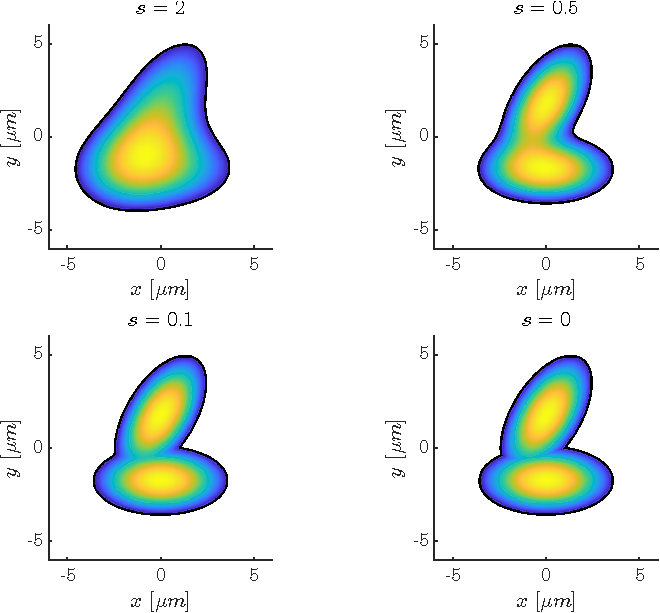
\includegraphics[width=0.8\textwidth]{chapter2/figures/compareSmoothness.pdf}
    \caption{Two ellipses blended with various values of smoothness $s$. The bottom right 
             figure is computed using standard minimum instead of smoothmin. Indeed,
             as $s \rightarrow 0$, the plot looks less smoothed across.}
    \label{fig:compareSmoothness}
\end{figure}
Figure \ref{fig:compareSmoothness} shows the effect of using different values of smoothness
$s$. Ultimately, using smoothmin was abandoned in favour or the computationally quicker \codeword{min},
which does not require the costly evaluation of the natural log and exponential functions.
\\

As shown in figure \ref{fig:mitosisplot}, we have a smooth splitting of a 
cell as the parameter $d$ ranges from $0.0$ to $9.1 \ \mu m$. Here $s$ is the 
smoothing parameter. In order to ensure that only the interior
of the SDF level section was plotted, I set positive entries to \codeword{nan},
which is MATLAB code for \textit{not a number}. The surface plots in figure \ref{fig:mitosisplot}
were produced via the use of MATLAB's \codeword{surf} function which ignores \codeword{nan} entries
in the underlying $Z$ matrix. One additional transformation made before plotting, was to multiply by 
$-1$ to reflect the SDF about the level plane, achieving a positive value inside the biomass.
\begin{figure}[!htb]
    \centering
    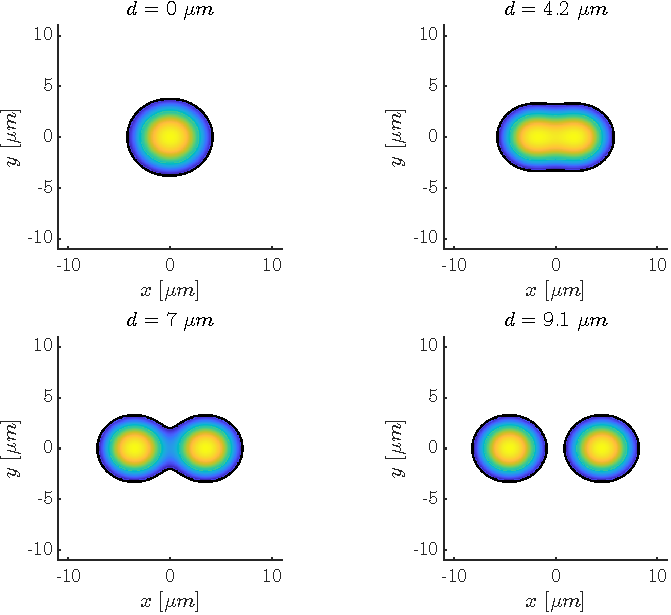
\includegraphics[width=0.8\textwidth]{chapter2/figures/mitosisPlot.pdf}
    \caption{The separation $d$ between two ellipse shapes with $s = 0.5$ and 
    an aspect ratio of $0.9$}
    \label{fig:mitosisplot}
\end{figure}
\\

A signed distance field for an ellipse is used to model Baker's yeast cells which
are in a pseudo-hyphal growth regime.
An ellipse centered at the origin with semi-major dimension $p$ (the $x$ intercept) and
semi-minor dimension $q$ (the $y$ intercept) has an SDF given by
\begin{equation*}
    f(x,y) = \sqrt{ \left( \frac{x}{p} \right)^2 + \left( \frac{y}{q} \right)^2 } - 1.
\end{equation*}
Recall that for computational efficiency we choose to use,
\begin{equation*}
    f(x,y) = \left( \frac{x}{p} \right)^2 + \left( \frac{y}{q} \right)^2  - 1.
\end{equation*}
This is not really a \textit{distance} field because it is 
dimensionless but it will still be called an SDF since it produces the 
elliptical shape all the same. We can also translate and rotate the ellipse, using
\begin{equation*} 
    \Delta \vb{x}' = 
    \begin{bmatrix}
        \cos{\theta} & \sin{\theta} \\
        -\sin{\theta} & \cos{\theta} 
    \end{bmatrix}
    \Delta \vb{x},
\end{equation*}
where $\Delta \vb{x} = (x-x_c) \hat{\vb{i}} + (y-y_c)\hat{\vb{j}} $ and $(x_c,y_c)$ is the
center of the ellipse. We call the components of $\Delta \vb{x} = \Delta x \hat{\vb{i}} +
\Delta y \hat{\vb{j}} $. The above trasnformation is a passive rotation because 
it rotates the whole SDF. The following equation
\begin{equation*}
    f(x,y) = \left[\frac{ (x-x_c)\cos{\theta} + (y-y_c) \sin{\theta}}{p} \right]^2 
        + \left[ \frac{-(x-x_c)\sin{\theta} +(y-y_c) \cos{\theta}}{q} \right]^2 - 1.
\end{equation*}
is used in the custom MATLAB function \codeword{ellipse.m} devloped here. Each individual 
cell has a unique value of $(x_c,y_c,p,q,\theta)$ which we index by $k$. Bringing them all 
together in one function using \codeword{min}, we have the colony SDF given by,
\begin{equation*}
    g(x,y) = \min_{k \in \{1, ..., N_{\textrm{cells}}\}} f_k(x,y),
\end{equation*}
where the individual SDF for each cell is given by 
\begin{equation*}
    \begin{split}
    f_k(x,y) &= \left[\frac{ (x-x_{c,k})\cos{\theta_k} + (y-y_{c,k}) \sin{\theta_k}}{p_k} \right]^2 \\ 
        &+ \left[ \frac{-(x-x_{c,k})\sin{\theta_k} +(y-y_{c,k}) \cos{\theta_k}}{q_k} \right]^2 - 1.
    \end{split}
\end{equation*}
Cell colonies can also be built up by combining the SDFs of the individual cells 
using a cumulative $\textrm{smoothmin}$.
\\

Some significant optimsations were made to make sure that the evalution of 
the colony SDF (evaluated via calling \codeword{ellipse.m}) was as fast as 
possible within the capabilities of MATLAB. These 
optimisations, which were crucial because \codeword{ellipse.m} is called per time step, 
are commented on in Chapter 2, subsection \ref{ssec:ellipse}.

\section{Cell colony dynamics with an underlying discrete network}
Now that we have introduced a robust mechanism to represent cell colony 
shape, the question naturally arises about how to represent the time dependence of this 
morphology. Baker's yeast grows via budding,
as shown in figure \ref{fig:yeastMicrograph}.
\begin{figure}[!htb]
    \centering
    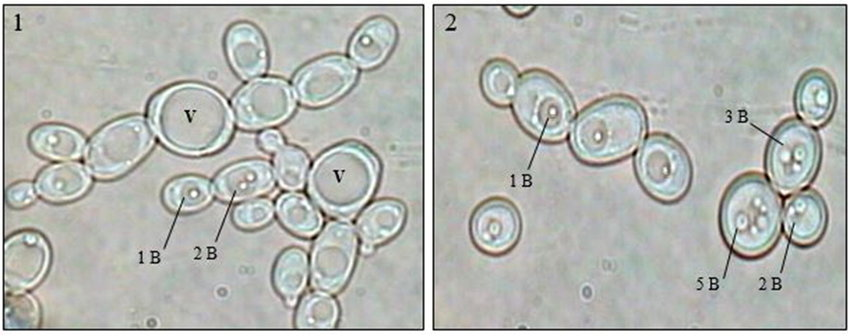
\includegraphics[width=0.8\textwidth]{chapter2/figures/yeastMicrograph.png}
    \caption{Micrographs of a translucent yeast strain studied
             in \cite{ebrahimi2020yeast}.}
    \label{fig:yeastMicrograph}
\end{figure}
To represent the branching dynamics of pseudo-hyphal yeast growth, 
an underlying discrete network which can change node count has been developed.
A colony for which the node count $N_{\textrm{nodes}}$ remains fixed is given 
by a undirected graph with adjacency matrix $A_{ij}$ where the edges are symbolically
represented by springs which model the elasticity of the cells. 
A diagram of this is shon in figure \ref{fig:yeastAsSpringNetwork}. 
\begin{figure}[!htb]
    \centering
    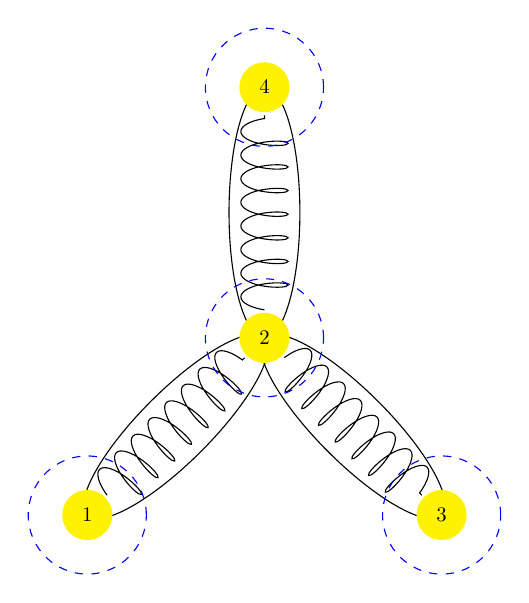
\begin{tikzpicture}
        \begin{scope}[scale=0.75,transform shape]
        \draw[rotate=45] (-0.5*4.243cm,0) ellipse (0.5*4.243cm and 0.6cm);
        \draw[rotate=-45] (0.5* 4.243,0) ellipse (0.5*4.243cm and 0.6cm);
        \draw[rotate=0] (0.0,0.5* 4.243)  ellipse (0.6cm and 0.5*4.243cm);
        
        \node[circle,fill=yellow, line width=1mm,inner sep=2.0mm] (a) at (-3,-3)  {1};
        \node[circle,fill=yellow, line width=1mm,inner sep=2.0mm] (b) at (0,  0)  {2};
        \node[circle,fill=yellow, line width=1mm,inner sep=2.0mm] (c) at (3, -3)  {3};
        \node[circle,fill=yellow, line width=1mm,inner sep=2.0mm] (d) at (0,4.243){4};
        \draw[decoration={aspect=0.3, segment length=3mm, amplitude=3mm,coil},decorate] (a) -- (b);
        \draw[decoration={aspect=0.3, segment length=3mm, amplitude=3mm,coil},decorate] (b) -- (c);  
        \draw[decoration={aspect=0.3, segment length=3mm, amplitude=3mm,coil},decorate] (b) -- (d); 

        \draw[dashed, color=blue]   (a)  ellipse (1.0cm and 1.0cm);
        \draw[dashed, color=blue]   (b)  ellipse (1.0cm and 1.0cm);
        \draw[dashed, color=blue]   (c)  ellipse (1.0cm and 1.0cm);
        \draw[dashed, color=blue]   (d)  ellipse (1.0cm and 1.0cm);
        \end{scope}
    \end{tikzpicture}
    
    \caption{A diagram of three elliptical cells with internal springs to represent biomass 
             elasticity ($\lambda_2 = \frac{K}{\eta \mu}$). The nodes are positioned at the ends of the major dimension
             of each ellipse and there are two nodes per cell. The force acting on 
             node $2$ for instance would be due to the forces from nodes $1$, $3$ and $4$.
             The dashed red circles represent the activation radius ($ \lambda_4 = R/L_0$) 
             of the contact force between the nodes.}
    \label{fig:yeastAsSpringNetwork}
\end{figure}

Relating the positions of the nodes in the network is done 
based on a simple implementation shown in figure \ref{fig:yeastMicrograph}.
\begin{figure}[!htb]
    \centering
    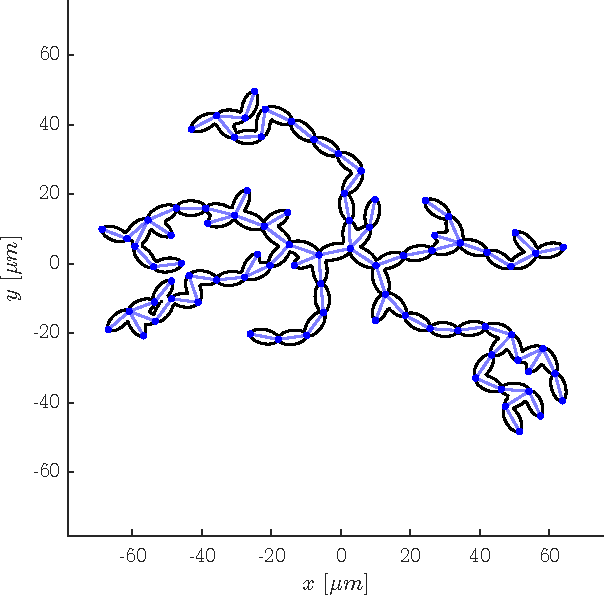
\includegraphics[width=0.6\textwidth]{chapter2/figures/networkYeast.pdf}
    \caption{A plot showing the underlying network of a simulated yeast colony 
            as well as the level-$0$ contour of the corresponding colony SDF.}
    \label{fig:yeastMicrograph}
\end{figure}
The equations that represent this correspondence between a cell indexed $k$ having 
parameters $(x_{c,k}, y_{c,k}, p_k, q_k, \theta_k)$
and its constitutive nodes indexed $i_1$ and $i_2$ are given by,
\begin{equation}
    p_k(t) = \frac{1}{2}||\vb{x}_{i_1} - \vb{x}_{i_2}||, \ 
    \textrm{where cell} \ k \ \textrm{is comprised of nodes} \ i_1, i_2, 
\end{equation}
\begin{equation}
    q_k(t) = \lambda_7 p_k(t), 
\end{equation}
\begin{equation}
    \theta_k(t) = \atan (y_{i_1} - y_{i_2},x_{i_1} - x_{i_2} ), 
\end{equation}
\begin{equation}
    \vb{x}_{c,k}(t) = \frac{1}{2} \left(\vb{x}_{i_1}(t) + \vb{x}_{i_2}(t)\right),
\end{equation}
where $\atan$ is the $2$ argument inverse tangent. In table \ref{table:perCellVariables} the variables 
associated with the cell indexed $k$, comprised of nodes $i_1$ and $i_2$ are summarised.

\begin{table}[!htb]
\begin{center}
    \begin{tabular}{ |c|c|c| } 
     \hline
      \textbf{Symbol} & \textbf{Formula in terms of nodes $i_1, i_2$} & \textbf{Description} \\ 
      \hline
     $\vb{x}_{c,k}$ & $\frac{1}{2} \left(\vb{x}_{i_1} + \vb{x}_{i_2}\right)$     & Center \\ 
     $p_k$          & $\frac{1}{2}||\vb{x}_{i_1} - \vb{x}_{i_2}||$                     & Semi-major radius \\ 
     $q_k$          & $\frac{\lambda_7}{2}||\vb{x}_{i_1} - \vb{x}_{i_2}||$                                      & Semi-minor radius \\         
     $\theta_k$     & $\atan (y_{i_1} - y_{i_2},x_{i_1} - x_{i_2} )$                   & Orintation angle \\         
     \hline   
    \end{tabular}   
\end{center}
\caption{The variables associated with each cell indexed $k$ and comprised of 
         nodes $i_1$ and $i_2$.}
\label{table:perCellVariables}
\end{table}

\section{The colony adjacency matrix, $A$}
In the software \codeword{CellColonySimulator} developed, the maximum 
number of nodes which the simulation can take is set to 
\codeword{maxNodeCount = 500}. This number is of course arbitrary and 
can be chosen to be much larger if the supercomputing time is available. 
In the case of figure \ref{fig:yeastAsSpringNetwork}, suppose
\codeword{maxNodeCount = 5}. Since there are only $4$ active nodes,
we would have an adjacency matrix of 
\begin{equation*}
    A = 
    \begin{bmatrix}
    0 & 1 & 0 & 0 & 0  \\
    1 & 0 & 1 & 1 & 0  \\
    0 & 1 & 0 & 0 & 0  \\
    0 & 1 & 0 & 0 & 0  \\
    0 & 0 & 0 & 0 & 0  \\ 
    \end{bmatrix},
\end{equation*}
which encodes the connectivity, i.e. node $1$ is connected to node $2$ and so on.
In order to represent the spring force from nodes $1$, $3$ and $4$ acting on node $2$,
we would sum up the spring forces from each connected node and apply Newton's Second Law, 
in the overdamped regime
\begin{equation*}
    \vb{v}_2 = \frac{\vb{F}_2}{\eta},
\end{equation*}
where $\vb{v}_2$ is the node 2's velocity, $\vb{F}_2$ is the net force acting on 
node 2, and $\eta$ is the dampening constant which is assumed to be uniform in the simulation.
The force on node 2 due to node 1 for example is given by $\vb{F}_{21}$ as 
\begin{equation*}
    \vb{F}_{21} = -K \left( ||\vb{x}_2 - \vb{x}_1|| - L_0 \right) \frac{\vb{x}_2 - \vb{x}_1}{||\vb{x}_2 - \vb{x}_1||},
\end{equation*}
which is Hooke's Law for a spring of stiffness $K$ and nominal length $L_0$.
The force acting on node 2 then is,
\begin{equation*}
    \vb{F}_{2} = \vb{F}_{21} + \vb{F}_{23} + \vb{F}_{24},
\end{equation*}
where the forces $\vb{F}_{23}$ and $\vb{F}_{24}$ are similarly defined. For a
system of nodes with arbitrary connectivty, the net force 
acting on node $i$ is given by 
\begin{equation*}
    \vb{F}_{i} = \sum_{j = 1, j \neq i}^{N_{\textrm{nodes}}} A_{ij} \vb{F}_{ij},
\end{equation*}
where $\vb{F}_{ij}$ is the spring force on node $i$ due to node $j$.
\\

In a very similar way, we add in a constant contact force between the nodes with radius $R \leq \frac{1}{2}L_0$,
which ensures that the nodes do not overlap. This is sometimes called an exclusion principle. The third 
type of force is in a sense an external driving force for the colony. It is a force 
proportional to the nutrient concentration gradient $\nabla c(\vb{x}_i, t)$ at the cell position. This type of 
force represents the attraction of the cells to areas of the petri dish with a high nutrient concentration.
A separate equation for the nutrient dynamics is introduced in section \ref{sec:nutrientField}. 
All of the three types of forces: elastic, contact and chemotaxis are added together to 
determine the motion of each node.
\begin{equation} \label{eqn:forcesNode_i}
    \begin{split}
        \frac{d \vb{x}_i}{dt} &= 
        \frac{K}{ \eta}\sum_{j = 1, j \neq i}^{N_{\textrm{nodes}}}   \left[ - A_{ij} \left( ||\vb{x}_i - \vb{x}_j|| - L_0\right) \frac{\vb{x}_i - \vb{x}_j}{||\vb{x}_i - \vb{x}_j||} \right]\\
         &+ \frac{F}{ \eta}\sum_{j = 1, j \neq i}^{N_{\textrm{nodes}}} \left[ H(R - ||\vb{x}_i - \vb{x}_j||) \frac{\vb{x}_i - \vb{x}_j}{||\vb{x}_i - \vb{x}_j||}     \right]\\ 
         &+ \frac{\gamma}{\eta} \nabla c (\vb{x}_i, t),
    \end{split}
\end{equation}
where $F$ is the magnitude of the contact force, and $\gamma$ is the magnitude of chemotaxis. In equation 
\ref{eqn:forcesNode_i} we have used the kinematic relationship $\vb{v}_i = \frac{d \vb{x}_i}{dt}$ and 
$H$ denotes a step function which is $0$ for a negative argument and $1$ for an arguemnt in 
$\mathbb{R}_{\geq 0}$.



\section{New cells from old}
We add in nodes at a small distance $\delta = 0.01$ beside old nodes 
which are taken to be parent nodes. The addition of new nodes is done in global mitosis events 
at time indices $n$ that are a multiple of
\begin{equation*}
    \Delta n = \bigg\lceil \frac{1}{\Delta t} \bigg\rceil,
\end{equation*}
where $\Delta t$ is the (non-dminesionalised) simulation time step, taken to be $0.01$ in \\
 \codeword{CellColonySimulator}.
The number of cells added at each global mitosis event reflects the exponential growth equation,
\begin{equation*}
    N_{\textrm{nodes}} = N_{0, \textrm{cell}} e^{t \mu(t)},
\end{equation*}
where the time-dependent growth rate $\mu$ is discussed 
in more detail in Chapter 2, subsection \ref{ssec:runSimulation}. The growth rate 
itself is given to be proportional to the average nutrient concentration over the node indices, and 
is given by equation \ref{eqn:growthRate}. This reflects the fact that if the nutrient has been depleted,
no new cells should be added, whereas if the nutrient has a uniform concentration of $1.0 \ \mu m^{-2}$ 
(taken to be the ideal nutrient concentration for growth and explained in section \ref{sec:nonDimEOMs}), 
then the colony will grow at the ideal growth rate, given by $\mu^*$.
\\

\begin{figure}[!htb]
    \centering
    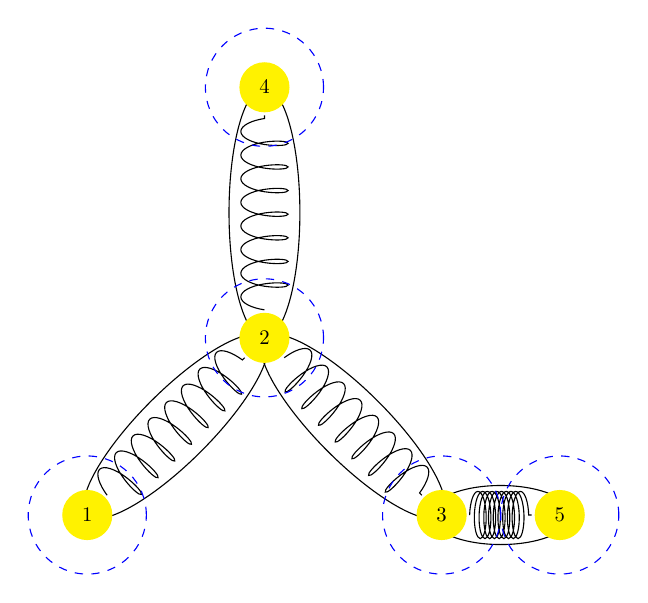
\begin{tikzpicture}
        \begin{scope}[scale=0.75,transform shape]
        \draw[rotate=45] (-0.5*4.243cm,0) ellipse (0.5*4.243cm and 0.6cm);
        \draw[rotate=-45] (0.5* 4.243,0) ellipse (0.5*4.243cm and 0.6cm);
        \draw[rotate=0] (0.0,0.5* 4.243)  ellipse (0.6cm and 0.5*4.243cm);
        \draw[rotate=0] (4.0,-3.0)  ellipse (1.2cm and 0.5cm);

        \node[circle,fill=yellow, line width=1mm,inner sep=2.0mm] (a) at (-3,-3)  {1};
        \node[circle,fill=yellow, line width=1mm,inner sep=2.0mm] (b) at (0,  0)  {2};
        \node[circle,fill=yellow, line width=1mm,inner sep=2.0mm] (c) at (3, -3)  {3};
        \node[circle,fill=yellow, line width=1mm,inner sep=2.0mm] (d) at (0,4.243){4};
        \node[circle,fill=yellow, line width=1mm,inner sep=2.0mm] (e) at (5,-3){5};
        \draw[decoration={aspect=0.3, segment length=3mm, amplitude=3mm,coil},decorate] (a) -- (b);
        \draw[decoration={aspect=0.3, segment length=3mm, amplitude=3mm,coil},decorate] (b) -- (c);  
        \draw[decoration={aspect=0.3, segment length=3mm, amplitude=3mm,coil},decorate] (b) -- (d); 
        \draw[decoration={aspect=0.3, segment length=0.6mm, amplitude=3mm,coil},decorate] (c) -- (e); 

        \draw[dashed, color=blue]   (a)  ellipse (1.0cm and 1.0cm);
        \draw[dashed, color=blue]   (b)  ellipse (1.0cm and 1.0cm);
        \draw[dashed, color=blue]   (c)  ellipse (1.0cm and 1.0cm);
        \draw[dashed, color=blue]   (d)  ellipse (1.0cm and 1.0cm);
        \draw[dashed, color=blue]   (e)  ellipse (1.0cm and 1.0cm);
        \end{scope}
    \end{tikzpicture}
    \caption{A mitosis event occurs via the addition of new nodes connected to old nodes.
             The nodes are added very close (distance $\delta \ll 1$) by the original nodes (exaggerated here)
             so that the spring force can be defined. After this point, 
             the initially compressed cell ``grows" outwards to achieve its nominal length, under 
             the influence of elasticity, contact and chemotactic forces.}
    \label{fig:addingACell}
\end{figure}
Figure \ref{fig:addingACell}, demonstrates the mechanism by which a new node is added to the 
colony, in this case, node $5$. The colony connectivity of this new $5$-node network would be given as 
\begin{equation*}
    A' = 
    \begin{bmatrix}
    0 & 1 & 0 & 0 & 0  \\
    1 & 0 & 1 & 1 & 0  \\
    0 & 1 & 0 & 0 & 1  \\
    0 & 1 & 0 & 0 & 0  \\
    0 & 0 & 1 & 0 & 0  \\ 
    \end{bmatrix},
\end{equation*}
because node $5$ is connected to node $3$. We mention that the new colony 
is defined by a different equilibrium position (when the time-derivative of 
position is quasi-steady).



\section{Incorporating the nutrient field} \label{sec:nutrientField}
A nutrient medium containing glucose is assumed to be given by a reaction-diffusion 
partial differential equation. That is the nutrient concentration $c(x,y,t)$ is given by
\begin{equation*}
    \pdv{c(x,y,t)}{t} = D \left( \frac{\partial^2 c(x,y,t)}{\partial x^2} + 
                          \frac{\partial^2 c(x,y,t)}{\partial y^2} \right) - r c(x,y,t) b(x,y,t)
\end{equation*}
where $b(x,y,t)$ is the microscopic biomass density of the cell colony, $D$ is a diffusion
coefficient and $r$ is a constant measuring the rate at which the cells consume nutrient.
The biomass field $b(x,y,t)$ is given as a function of the colony SDF as,
\begin{equation*}
    b(x,y,t) = \begin{cases}
                -g(x,y,t), & \ \textrm{if} \ g(x,y,t) \leq 0, \\
                0,         & \ \textrm{otherwise}.
               \end{cases}
\end{equation*}
In the case of the plotting of $b(x,y,t)$ we use \codeword{nan} instead of $0$. 
\\

The PDE is subjected to the Dirichlet condition
that the nutrient density takes a value of $1.0$ at the boundary. In order to simulate the nutrient field
numerically a foward time centered space (FTCS) scheme was prototyped on the square grid 
covering the domain. However, this scheme was found to be numerically unstable
for small spatial steps $h$ and large time steps $\Delta t$ and was discarded
in favour of the unconditionally numerically stable Crank-Nicholson scheme detailed
in section \ref{Crank_Nicholson}. Before this is possible, 
we carry out the non-dimensionalising of the equations of motion (EOMs).


\section{Non-dimensionalising the equations of motion}\label{sec:nonDimEOMs}

In order to non-dimensionalise the equations of motion (EOMs) we
introduce dimensionless parameters $\vb{x}_i = X\hat{\vb{x}}_i$, $t = T \hat{t}$, $b = B \hat{b}$
and $c = G \hat{c}$, where $X, T, B$ and $G$ are general undetermined scalings for the independent 
and dependent variables, respectively. At the outset, we fix $X = L_0 = 7.5 \ \mu m$ the nominal major cell diameter
found by \cite{chavez2024cell}. The same source gives an aspect ratio
of $7.5 \times 5.5 \ \mu m$ which we call $\lambda_7 = \frac{q}{p}$. The reason for the numbering 
will become clear from the non-dimensionalisation of the model. The time scale is chosen as
$T = \frac{1}{\mu^*}$ the reciprocal of specific growth rate for yeast, that is the $\mu^* = \mu(0)$ that appears in
the formula for the total node count. The value chosen was $\mu^* = 0.46$ hour$^{-1}$
from the value cited at \cite{salari2017investigation} which represents ideal conditions
for saccharomyces cerevisiae growth on a synthetic culture medium containing glucose. 
The value given by (\cite{salari2017investigation}) is a doubling rate of $90$ mins. In the model
presented in this thesis, that amounted to $\mu^* = \frac{\log(2)}{1.5 \ \textrm{hours}} = 0.4621$ hour$^{-1}$ which
was rounded down to $0.46$ hour$^{-1}$ as a conservative estimate.

\begin{table}[!htb]
\begin{center}
    \begin{tabular}{ |c|c|c| } 
     \hline
      \textbf{Symbol} & \textbf{Value} & \textbf{Descriptive name} \\ 
      \hline
     $L_0$   & $7.5 \ \mu m$       & Average cell length \\ 
     $\mu^*$ & $0.46$ hour$^{-1}$   & Ideal growth rate  \\ 
     $c_0$   & $1.0 \ \mu m^{-2}$  & Nutrient concentration \\ 
     \hline
     
    \end{tabular}
    
\end{center}
\caption{A summary of the numerical units}
\label{table:NumericalUnits}
\end{table}

It is necessary to point out that initial concentration, the choice for $G = c_0$, is 
typically measured in mol$\cdot \mu m^{-2}$ which amounts to Avagadro's number of 
glucose molecules per $\mu m^{2}$. In our case, we choose a number $N_G$ such that 
the concentration comes out to $1.0 \ N_G \cdot \mu m^{-2}$. We always
omit the $N_G$ because it is of no consequence dimensionally.
Also useful to recapitulate, is the formula for the total node count,
\begin{equation}  
    N_{\textrm{nodes}}(t) = N_{\textrm{cells},0} e^{ t \mu^* \hat{\mu}(t)},
\end{equation}
where $N_{\textrm{cells},0} = 1$ because we always begin with a single cell,
and $\hat{\mu}(t)$ is the unitless growth rate. Note that
$\mu(t) = \mu^* \hat{\mu}(t)$ and that $\hat{\mu}(0) = 1.0$.
This equation is used in the computation of $\mu^*$ based on the doubling time
provided in \cite{salari2017investigation}.
Hopefully it is clear that
the values of $L_0, \mu^*, c_0$
can be changed to fit different species of fungus. Those values given here
are just representative and further controlled experimental studies would 
need to be done to verify them.

\subsection{Non-dimensionalising the nutrient PDE}

Substituting these parameters into the reaction-diffusion PDE for nutrient concentration, we obtain 
\begin{equation*}
    \frac{c_0}{(1/\mu^*)}\pdv{\hat{c}}{\hat{t}} = \left(\frac{D c_0}{ L_0^2} \right)\left(\pdv[2]{\hat{c}}{\hat{x}} + \pdv[2]{\hat{c}}{\hat{y}} \right) -
      \left( r c_0 B\right)  \hat{c}\hat{b},
\end{equation*}
which results in 
\begin{equation*}
    \pdv{\hat{c}}{\hat{t}} = \left(\frac{D}{ \mu^* L_0^2} \right)\left(\pdv[2]{\hat{c}}{\hat{x}} + \pdv[2]{\hat{c}}{\hat{y}} \right) -
      \left( \frac{r  B}{\mu^*}\right)  \hat{c}\hat{b}.
\end{equation*}
Call the dimensionless diffusion constant $\lambda_1 = \frac{D}{ \mu^* L_0^2}$ and 
set $\frac{r  B}{\mu^*}=1$ which are free to do since $B$ is unset to begin with. This means 
that the scaling for the biomass density is $B = \frac{\mu^*}{r}$. The reaction diffusion equation 
reduces to 
\begin{equation*}
    \pdv{\hat{c}}{\hat{t}} = \lambda_1 \left(\pdv[2]{\hat{c}}{\hat{x}} + \pdv[2]{\hat{c}}{\hat{y}} \right) -
      \hat{c}\hat{b}.
\end{equation*}

\subsection{Non-dimensionalising the nodes ODE}
Now, for the EOM for the nodes, we have
\begin{equation*}
    \begin{split}
        \frac{d \vb{x}_i}{dt} &= 
        \frac{K}{ \eta}\sum_{j = 1}^N   \left[ - A_{ij} \left( ||\vb{x}_i - \vb{x}_j|| - L_0\right) \frac{\vb{x}_i - \vb{x}_j}{||\vb{x}_i - \vb{x}_j||} \right]\\
         &+ \frac{F}{ \eta}\sum_{j = 1}^N \left[ H(R - ||\vb{x}_i - \vb{x}_j||) \frac{\vb{x}_i - \vb{x}_j}{||\vb{x}_i - \vb{x}_j||}     \right]\\ 
         &+ \frac{\gamma}{\eta} \nabla c (\vb{x}_i, t).
    \end{split}
\end{equation*}
Substituting the dimensionless parameters, we acquire
\begin{equation*}
    \begin{split}
        \frac{L_0}{(1/\mu^*)}\frac{d \hat{\vb{x}}_i}{d \hat{t}} &= 
        \frac{K L_0}{ \eta}\sum_{j = 1, j \neq i}^N   \left[ - A_{ij}\left( ||\hat{\vb{x}}_i - \hat{\vb{x}}_j|| -  1\right) \frac{\hat{\vb{x}}_i - \hat{\vb{x}}_j}{||\hat{\vb{x}}_i - \hat{\vb{x}}_j||} \right]\\
         &+ \frac{F}{  \eta}\sum_{j = 1, j \neq i}^N \left[H(\hat{R} - ||\hat{\vb{x}}_i - \hat{\vb{x}}_j||) \frac{\hat{\vb{x}}_i - \hat{\vb{x}}_j}{||\hat{\vb{x}}_i - \hat{\vb{x}}_j||}     \right]\\ 
         &+ \frac{\gamma C}{ \eta L_0} \hat{\nabla}  \hat{c} (\hat{\vb{x}}_i, \hat{t}),
    \end{split}
\end{equation*}
which, after rearranging, becomes,
\begin{equation*}
    \begin{split}
        \frac{d \hat{\vb{x}}_i}{d \hat{t}} &= 
        \frac{K}{ \eta \mu^*}\sum_{j = 1, j \neq i}^N   \left[ - A_{ij}\left( ||\hat{\vb{x}}_i - \hat{\vb{x}}_j|| -  1\right) \frac{\hat{\vb{x}}_i - \hat{\vb{x}}_j}{||\hat{\vb{x}}_i - \hat{\vb{x}}_j||} \right]\\
         &+ \frac{F}{  \eta \mu^* L_0}\sum_{j = 1, j \neq i}^N \left[H(\hat{R} - ||\hat{\vb{x}}_i - \hat{\vb{x}}_j||) \frac{\hat{\vb{x}}_i - \hat{\vb{x}}_j}{||\hat{\vb{x}}_i - \hat{\vb{x}}_j||}     \right]\\ 
         &+ \frac{\gamma C}{ \eta \mu^* L_0^2} \hat{\nabla}  \hat{c} (\hat{\vb{x}}_i, \hat{t}).
    \end{split}
\end{equation*}
Only one of the coefficients could be set to unity, but instead we choose $C = c_0 = 1$ to be the initial 
concentration. That leaves us with four additional parameters,
\begin{equation*}
    \lambda_2 = \frac{K}{ \eta \mu^*},
\end{equation*}
\begin{equation*}
    \lambda_3 = \frac{F}{  \eta \mu^* L_0},
\end{equation*}
\begin{equation*}
    \lambda_4 = \frac{R}{L_0},
\end{equation*}
\begin{equation*}
    \lambda_5 = \frac{\gamma c_0}{ \eta \mu^*L_0^2}.
\end{equation*}

\subsection{Non-dimensionalising the biomass equation}
The field $g(x,y,t) = \hat{g}(\hat{x},\hat{y},\hat{t})$ is unitless 
so we are left with the following EOM for the biomass field,
\begin{equation*}
    B\hat{b} = \begin{cases}
                -  \hat{g}(\hat{x},\hat{y},\hat{t}), & \ \textrm{if} \ \hat{g}(\hat{x},\hat{y},\hat{t}) \leq 0, \\
                    0, &    \ \textrm{otherwise}.
               \end{cases}
\end{equation*}
\begin{equation*}
    \hat{b} = \begin{cases}
                -  \frac{r}{\mu^*}\hat{g}(\hat{x},\hat{y},\hat{t}), & \ \textrm{if} \ \hat{g}(\hat{x},\hat{y},\hat{t}) \leq 0, \\
                    0, &    \ \textrm{otherwise}.
               \end{cases}
\end{equation*}
which leaves us with an additional parameter, $\lambda_6 =\frac{r}{\mu^*}$. The final model parameter is the cell aspect ratio, $\lambda_7$.
The model parameters are summarised in table \ref{table:VariableNames}.


\begin{table}[!htb]
\begin{center}
    \begin{tabular}{ |c|c|c| } 
     \hline
      \textbf{Symbol} & \textbf{Expression} & \textbf{Descriptive name} \\ 
      \hline
     $\lambda_1$ & $\frac{D}{ \mu^* L_0^2}$ & diffusivity \\ 
     $\lambda_2$ & $\frac{K}{ \eta \mu^*}$ & elasticity \\ 
     $\lambda_3$ & $\frac{F}{  \eta \mu^* L_0}$ & respulsivity \\ 
     $\lambda_4$ & $\frac{R}{L_0}$ & respulsion radius \\ 
     $\lambda_5$ & $\frac{\gamma c_0}{ \eta \mu^* L_0^2}$ & mobility \\ 
     $\lambda_6$ & $\frac{r}{\mu^*}$ & metabolic rate \\ 
     $\lambda_7$ & $\frac{\textrm{cell minor axis}}{\textrm{cell major axis}} = \frac{2q}{2p}$ & cell aspect ratio \\ 
     \hline
     
    \end{tabular}
    
\end{center}
\caption{A summary of the dimensionless model parameters}
\label{table:VariableNames}
\end{table}


\subsection{Non-dimensional model equations of motion (EOMs)}

Dropping the hats on variable symbols, we arive at the final system equations of motion which
span from equation \ref{eqn:EOMs_PDE} to \ref{eqn:centerPos}.


\begin{equation} \label{eqn:EOMs_PDE}
    \boxed{\pdv{c}{t} = \lambda_1 \left(\pdv[2]{c}{x} + \pdv[2]{c}{y} \right) - bc,
     \ \textrm{for} \ (x,y) \in \Omega \setminus \partial \Omega,}
\end{equation}
\begin{equation}
    \boxed{c(x,y,t) = 1.0, \ \textrm{for} \ (x,y) \in \partial \Omega,}
\end{equation}
\begin{equation}
    \boxed{c(x,y,0) = 1.0,}
\end{equation}
\begin{equation}\label{eqn:EOMs_ODE}
    \boxed{
    \begin{split}
        \frac{d \vb{x}_i}{d t} 
         &= \lambda_2 \sum_{j=1}^{N_{\textrm{nodes}}} \left[ A_{ij}\left( 1- ||\vb{x}_i - \vb{x}_j|| \right) \frac{\vb{x}_i - \vb{x}_j}{||\vb{x}_i - \vb{x}_j||} \right]\\
         &+ \lambda_3 \sum_{j=1}^{N_{\textrm{nodes}}} \left[H(\lambda_4 - ||\vb{x}_i - \vb{x}_j||) \frac{\vb{x}_i - \vb{x}_j}{||\vb{x}_i - \vb{x}_j||}     \right]\\ 
         &+ \lambda_5 \nabla c (\vb{x}_i, t), \ \textrm{for} \ i \in \{ 1, ...,N_{\textrm{nodes}} \},  
    \end{split}}
\end{equation}
\begin{equation}
    \boxed{\vb{x}_1(0) = (0.5 \cos{\Theta_e}, 0.5 \sin{\Theta_e}), \ \vb{x}_2(0) = (-0.5 \cos{\Theta_e}, -0.5 \sin{\Theta_e}), }
\end{equation}
\begin{equation} \label{eqn:expGrowth}
    \boxed{N_{\textrm{nodes}} = N_{0, \textrm{cells}} e^{t \mu(t)}, \textrm{where} \ N_{0, \textrm{cells}} = 1, }
\end{equation}
\begin{equation}\label{eqn:growthRate}
    \boxed{\mu(t) = \frac{1}{N_{\textrm{nodes}}}\sum_{i=1}^{N_{\textrm{nodes}}} c(\vb{x}_i, t), } 
\end{equation}
\begin{equation} \label{eqn:biomass}
    \boxed{
    b(x,y,t) = 
    \begin{cases}
        -\lambda_6 g(x,y,t), & \ \textrm{if} \ g(x,y,t) \leq 0, \\
            0, &    \ \textrm{otherwise},
    \end{cases}
    }
\end{equation}
\begin{equation}
    \boxed{
    g(x,y,t) = \min_{k \in \{  1, ..., N_{\textrm{cells}}\}} f_k (x,y,t),
    }
\end{equation}
\begin{equation}
    \boxed{
    \begin{split}
    f_k(x,y,t) &= \left[\frac{ (x-x_{c,k}(t))\cos{\theta_k} + (y-y_{c,k}(t)) \sin{\theta_k}}{p_k(t)} \right]^2 \\ 
               &+ \left[ \frac{-(x-x_{c,k}(t))\sin{\theta_k} +(y-y_{c,k}(t)) \cos{\theta_k}}{q_k(t)} \right]^2 - 1,
    \end{split}
    }
\end{equation}
\begin{equation}\label{eqn:semiMajorAxis}
    \boxed{p_k(t) = \frac{1}{2}||\vb{x}_{i_1} - \vb{x}_{i_2}||, \ 
    \textrm{where cell} \ k \ \textrm{is comprised of nodes} \ i_1, i_2,} 
\end{equation}
\begin{equation}\label{eqn:semiMinorAxis}
    \boxed{q_k(t) = \lambda_7 p_k(t), }
\end{equation}
\begin{equation}\label{eqn:orientationAngle}
    \boxed{\theta_k(t) = \atan (y_{i_1} - y_{i_2},x_{i_1} - x_{i_2} ), }
\end{equation}
\begin{equation} \label{eqn:centerPos}
    \boxed{ \vb{x}_{c,k}(t) = \frac{1}{2} \left(\vb{x}_{i_1}(t) + \vb{x}_{i_2}(t)\right). }
\end{equation}

Note that $i$ and $j$ index over node numbers, $k$ over cells, and $i_1$ and $i_2$ denote the nodes
that comprise cell $k$. Also note that $\Theta_e$, the orientation of the starting cell
is chosen to be different for each ensemble instance $e$. In fact,
this is chosen to be a uniform random number between $[0,2\pi]$ which
is unpdated in the loop over the ensemble in \codeword{Master.m} as part of the \textbf{CellColonySimulator}
MATLAB software.
Finally the petri-dish domain is given by 

\begin{equation}
    \boxed{\Omega = \left[-\frac{1}{2}L_{\textrm{petri-dish}},\frac{1}{2}L_{\textrm{petri-dish}} \right] \times
             \left[-\frac{1}{2}L_{\textrm{petri-dish}},\frac{1}{2}L_{\textrm{petri-dish}} \right] \subset \mathbb{R}^2,}
\end{equation}
where it is noted that $L_{\textrm{petri-dish}}$ is unitless.


\section{Numerically solving for the nutrient field} \label{Crank_Nicholson}
In order to advance the nutrient field in time, an efficient and stable numerical solver
was required. Because of the fact that the nutrient field $c(x,y,t)$ is coupled 
to the biomass field which is dependent on a discrete network that changes in connectivity and 
node count, it was necessary to implement the method in-house, as opposed to 
using a pre-existing MATLAB boundary value solver for instance. The Crank-Nicolson method (\cite{crank1947practical}) was 
chosen for the practical reason that it led to faster simulations overall since a larger
time step could be used as opposed to the explicit forward in time central in space (FTCS) scheme. This 
is a direct consequence of the fact that the (implicit) Crank-Nicholson scheme is unconditionally numerically 
stable. Let us begin by verifying this fact using the what is
known as Von Neumann stability analysis (\cite{charney1950numerical}).
\begin{figure}[!htb]
    \centering
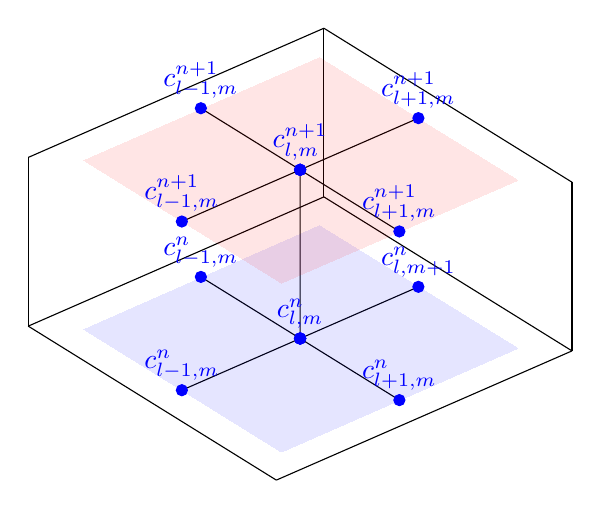
\begin{tikzpicture}
    \pgfplotsset{every tick label/.append style={font=\scriptsize}}
 
    \begin{axis}[view = {50}{50},
        width=0.7\textwidth,
        xmax = 10,
        xmin = -10,
        ymax = 10, 
        ymin = -10, 
        zmax = 10, 
        zmin = 0,
        xtick=\empty,
        ytick=\empty,
        ztick=\empty,
        grid,
        grid style={dashed,gray!40},
        3d box=background]
     
        \addplot3[mark=*,black,mark options={blue},point meta=explicit symbolic,nodes near coords] 
        coordinates 
        {
            (0,0,0) [$c_{l,m}^n$]
            (-8,0,0)[$c_{l-1,m}^n$]
            (0,0,0)
            (8,0,0)[$c_{l+1,m}^n$]
            (0,0,0)
            (0,8,0)[$c_{l,m+1}^n$]
            (0,0,0)
            (0,-8,0)[$c_{l-1,m}^n$]
            (0,0,0)
            (0,0,10)[$c_{l,m}^{n+1}$]
            (-8,0,10)[$c_{l-1,m}^{n+1}$]
            (0,0,10)
            (8,0,10)[$c_{l+1,m}^{n+1}$]
            (0,0,10)
            (0,8,10)[$c_{l+1,m}^{n+1}$]
            (0,0,10)
            (0,-8,10)[$c_{l-1,m}^{n+1}$]
        };

        \addplot3 [
        domain = -8:8,
        domain y = -8:8,
        samples = 2,
        samples y = 2,
        surf,
        fill opacity=0.1,
        shader = interp] {0};

        \addplot3 [
        domain = -8:8,
        domain y = -8:8,
        samples = 2,
        samples y = 2,
        surf,
        fill opacity=0.1,
        color=red,
        shader = interp] {10};
     
    \end{axis}
     
\end{tikzpicture}
\caption{The five point stencil for the nutrient field at times $t_{n} = n \Delta t$ (blue plane)
         and $t_{n+1} = (n+1) \Delta t$ (red plane) used for the Crank-Nicolson scheme on the domain
         interior.}
\label{fig:CrankNicolsonScheme}
\end{figure}

Firstly, we 
define the nutrient field as $c_{l,m}^{n} = c(x_l, y_m, t_n)$, where $x_l = -\frac{1}{2}L_{\textrm{petri-dish}} + h l$, 
$y_m = -\frac{1}{2}L_{\textrm{petri-dish}} + h m$ and similarly for $b_{l,m}^{n}$,
the biomass. The values  $c_{l,m}^{n}$ precisely satisfy the discretised equations which follow.
Let  $\bar{c}_{l,m}^{n}$ be the solution achieved with finite precison arithmetic 
operations which does not necessarily satisfy the equations, up to some error term,
\begin{equation*}
    \epsilon_{l,m}^n = \bar{c}_{l,m}^{n} - c_{l,m}^{n}.
\end{equation*}
Carrying out the Crank-Nicolson discretisation with the values $c_{l,m}^{n}$, we derive
\begin{equation*}
    \frac{c_{l,m}^{n+1} - c_{l,m}^{n}}{\Delta t} =
    \frac{\lambda_1}{2} \left( \nabla^2 c_{l,m}^{n+1} + \nabla^2 c_{l,m}^{n} \right) -
     \frac{1}{2} b_{l,m}^{n} (c_{l,m}^{n+1} + c_{l,m}^{n}).
\end{equation*}
The laplacian terms here are calculated with a five-point stencil at the current and subsequent 
time steps as shown in figure \ref{fig:CrankNicolsonScheme}. This results in the following discretisation,

\begin{equation*}
    \begin{split}
        \frac{c_{l,m}^{n+1} - c_{l,m}^{n}}{\Delta t} &=
        \frac{\lambda_1}{2}  \left( \frac{c_{l+1,m}^{n+1} - 2 c_{l,m}^{n+1} + c_{l-1,m}^{n+1} }{h^2} + 
                                    \frac{c_{l,m+1}^{n+1} - 2 c_{l,m}^{n+1} + c_{l,m-1}^{n+1} }{h^2} \right)  \\
                                   & +\frac{\lambda_1}{2} \left( \frac{c_{l+1,m}^{n} - 2 c_{l,m}^{n} + c_{l-1,m}^{n} }{h^2} + 
                                    \frac{c_{l,m+1}^{n} - 2 c_{l,m}^{n} + c_{l,m-1}^{n} }{h^2} \right) \\
                                   &-\frac{1}{2} b_{l,m}^{n} (c_{l,m}^{n+1} + c_{l,m}^{n}).
    \end{split}
\end{equation*}
To evaluate the numerical stability, we introduce a constant $\alpha = \frac{ \lambda_1 \Delta t }{h^2}$.
With this constant in place, we continue with
\begin{equation*}
    \begin{split}
        c_{l,m}^{n+1} - c_{l,m}^{n} &=
       \frac{\alpha}{2}  \left( c_{l+1,m}^{n+1} + c_{l-1,m}^{n+1} + 
                       c_{l,m+1}^{n+1} + c_{l,m-1}^{n+1}  \right) - 2 \alpha c_{j,k}^{n+1}  \\
                                   & +\frac{\alpha}{2} \left( c_{l+1,m}^{n}+ c_{l-1,m}^{n} + 
                                    c_{l,m+1}^{n} + c_{l,m-1}^{n}  \right) - 2 \alpha c_{l,m}^{n} \\
                                   &-\frac{\Delta t}{2} b_{l,m}^{n} (c_{l,m}^{n+1} + c_{l,m}^{n}).
    \end{split}
\end{equation*}
Since the discretised equations are linear in $c_{l,m}^{n}$ (taking $b_{l,m}^{n}$ to be slowly varying)
and since $\bar{c}_{l,m}^n$ also form a solution, the $\epsilon_{l,m}^n$ are also 
a solution.
\begin{equation*}
    \begin{split}
        \epsilon_{l,m}^{n+1} - \epsilon_{l,m}^{n} &=
       \frac{\alpha}{2}  \left( \epsilon_{l+1,m}^{n+1} + \epsilon_{l-1,m}^{n+1} + 
                                \epsilon_{l,m+1}^{n+1} + \epsilon_{l,m-1}^{n+1}  \right) - 2 \alpha \epsilon_{l,m}^{n+1}  \\
                                   & +\frac{\alpha}{2} \left( \epsilon_{l+1,m}^{n}+ \epsilon_{l-1,m}^{n} + 
                                   \epsilon_{l,m+1}^{n} + \epsilon_{l,m-1}^{n}  \right) - 2 \alpha \epsilon_{l,m}^{n} \\
                                   &-\frac{\Delta t}{2} b_{l,m}^{n} (\epsilon_{l,m}^{n+1} + \epsilon_{l,m}^{n}).
    \end{split}
\end{equation*}
We subsitute in an ansatz for the error term which is standard in Von Neumann stability analysis, namely
\begin{equation*}
    \epsilon_{l,m}^n = \xi^n e^{i \nu_x l h} e^{i \nu_y m h},
\end{equation*}
where $\nu_x$ and $\nu_y$ are wavenumbers and $h$ is the spatial step. Note that $i = \sqrt{-1}$. In order for the numerical
method to be stable, we require that $|\xi| \leq 1$ for all values of the wavenumbers $\nu_x, \nu_y$.
Substituting this expression into the discretised equation for the error, we get,
\begin{equation*}
    \begin{split}
        \xi^{n+1} e^{i \nu_x l h} e^{i \nu_y m h} - \xi^{n} e^{i \nu_x l h} e^{i \nu_y m h} &=
       \frac{\alpha}{2}  \left( \xi^{n+1} e^{i \nu_x (l+1) h} e^{i \nu_y m h} + \xi^{n+1} e^{i \nu_x (l-1) h} e^{i \nu_y m h} \right) \\
       &+ \frac{\alpha}{2}\left( \xi^{n+1} e^{i \nu_x l h} e^{i \nu_y (m+1) h} + \xi^{n+1} e^{i \nu_x l h} e^{i \nu_y (m-1) h}  \right) \\
       &-2 \alpha\xi^{n+1} e^{i \nu_x l h} e^{i \nu_y m h}  \\
       &+\frac{\alpha}{2} \left( \xi^{n} e^{i \nu_x (l+1) h} e^{i \nu_y k h}+ \xi^{n} e^{i \nu_x (m-1) h} e^{i \nu_y m h}\right) \\
       &+ \frac{\alpha}{2}\left(\xi^{n} e^{i \nu_x l h} e^{i \nu_y (k+1) h} + \xi^{n} e^{i \nu_x m h} e^{i \nu_y (m-1) h}  \right) \\
       &-2 \alpha \xi^{n} e^{i \nu_x l h} e^{i \nu_y k h}\\
       &-\frac{\Delta t}{2} b_{l,m}^{n} (\xi^{n+1} e^{i \nu_x l h} e^{i \nu_y m h} + \xi^{n} e^{i \nu_x l h} e^{i \nu_y m h}).
    \end{split}
\end{equation*}
Dividing through by $\xi^{n} e^{i \nu_x l h} e^{i \nu_y m h}$, we attain,
\begin{equation*}
    \begin{split}
        \xi - 1 &=
       \frac{\alpha}{2}  \left( \xi e^{i \nu_x h}+ \xi e^{-i \nu_x h} \right) 
       + \frac{\alpha}{2}\left( \xi  e^{i \nu_y h} + \xi  e^{-i \nu_y h}  \right) 
       -2 \xi \alpha  \\
       &+\frac{\alpha}{2} \left(  e^{i \nu_x  h}+  e^{-i \nu_x h}\right)
       + \frac{\alpha}{2}\left(   e^{i \nu_y h} +   e^{-i \nu_y  h}  \right) 
       -2 \alpha
       -\frac{\Delta t}{2} b_{l,m}^{n} (\xi + 1).
    \end{split}
\end{equation*}
Using the fact that $ \frac{e^{i \nu_x h}+  e^{-i \nu_x h}}{2} = \cos(\nu_x h)$ and similarly for
the other terms, we have,
\begin{equation*}
    \begin{split}
        \xi - 1 &=
         \alpha \xi \cos(\nu_x h) 
       + \alpha \xi \cos(\nu_y h) 
       -2 \alpha \xi   \\
       &+\alpha \cos(\nu_x h) 
       + \alpha \cos(\nu_y h) 
       -2 \alpha
       -\frac{\Delta t}{2} b_{l,m}^{n} (\xi + 1).
    \end{split}
\end{equation*}
Finally, solving for $\xi$, and taking its absolute value we have,
\begin{equation*}
    |\xi| = \left| \frac{1 + \alpha \left[ \cos(\nu_x h) + \cos(\nu_y h) \right] - 2 \alpha -\frac{1}{2} \Delta t b_{l,m}^{n} }
                        {1 -\alpha \left[ \cos(\nu_x h) + \cos(\nu_y h) \right]  + 2 \alpha +\frac{1}{2} \Delta t b_{l,m}^{n}} \right|.
\end{equation*}
In order to complete the analysis, consider when biomass is $b_{l,m}^{n} = 0$. We have the simplified
equation,
\begin{equation*}
    |\xi| = \left| \frac{1 -\alpha(2 - \left[ \cos(\nu_x h) + \cos(\nu_y h) \right]) }
                        {1 +\alpha(2 - \left[ \cos(\nu_x h) + \cos(\nu_y h)\right])} \right|,
\end{equation*}
Which has a numerator less than or equal to $1$ because $\alpha > 0$ and 
$0 \leq 2 - \left[ \cos(\nu_x h) + \cos(\nu_y h) \right] \leq 4$. The denominator is 
always greater than or equal to $1$, which is enough to prove that
the Crank-Nicolson scheme for the standard heat equation is numerically stable.
\\
\\
Whether this generalises to non-zero $b_{l,m}^{n}$ is determined by numerical experiments, and 
indeed for $\alpha = \frac{\lambda_1 \Delta t}{h^2} = \frac{(0.1) (0.01)}{(0.1)^2} = 0.1$, the scheme 
was not found to be unstable. However, for higher values of $\alpha$ it was possible to see spurious 
oscillations in the solution field for $c$ which obviously suggests some form of instability.






% continue with as many chapter as required
\conclusions

\section{Summary remarks}
The components of this thesis when considered individually
are adapted from previous mathematical 
modelling, sometimes in biology, sometimes not. The value of 
what has been done emerges from the interplay of the elements
\begin{enumerate}
    \item A PDE nutrient field,
    \item An overdamped and growing spring network,
    \item A cell colony given as a level-section of a polynomial,
\end{enumerate}
all of which I feel were necessary for the model's overall 
synthesis to occur. I by no means believe 
that even a small proportion of the total causes and effects
have been accounted for in regard to baker's yeast proliferation 
in nutrient-poor conditions. But it is my hope 
that new model \textit{triple-points} or even \textit{multi-stable symbolic states} 
can be sought after in future 
studies.
\\

Qualitatively different types of models, when coupled
in this attentive way can give rise to new dynamics not found in 
any singular model. That being said, 
the process of learning and tending to more models than one can be
laborious, if not grounded in some sort of overarching 
framework, even if that framework is to disappear 
when the total project emerges.
\\

\section{A word on my scientific process}
The openness to testing different models without 
the promise of intellectual refuge in one prior form, came 
from my conviction that \textit{life itself} is irreducible
and heterogenous. Our mathematical models sometimes reflect 
this truth (that I have come to understand through struggle, 
hurt and loneliness), and sometimes 
they do not. In that sense, this thesis is a 
\textit{personal reckoning} with the very structuring 
force of our own assumptions. But there are other 
forces at play aswell.
\\

The pressure of scientific tradition was a necessary 
influence on my project, and so was 
my own opposing reaction to its reductionist tendancies.
Without these forces this project would not have 
branched out into what it became. Since 
I too am a living being whose cells 
are in constant interaction with the environment, 
it was necessary to bring my own subjectivity
into this tango of symbols.
\\

\section{Philosophical remarks}

\textit{The reader who is not philosophically inclined may ignore this.}
\\

\textit{O let us talk of quiet that we know,
that we can know, the deep and lovely quiet
of a strong heart at peace!}
\\
\textit{How can we this, our own quietus, make?}
\\
An excerpt from \textit{The Ship of Death}, by D.H.Lawrence.
\\

In classical mechanics, forces are vectors that 
are summed to give the net force. What we have 
come to forget is that individual forces themselves
could have different mathematical structures associated 
to them. There may be more natural or ergonomic 
formalisms associated to each force. 
The direct approach then, is to consider 
``force formalisms" that allow for designed trajectories.
\\

It seems, ``change how you look at it, and you will see something 
different,'' is a dismissal of form. That is not the case. 
There is a rich history of mathematics that studies 
subjectivity directly, but you can only see that if you sit with 
it for long enough. Mathematics is wedded to form and form 
is about perception.
\\

Like Lindenmayer systems, \textit{symbolic ideas} that undergo mutations
and dilutions often become what they are not. Is this a symptom 
of the nature of nature? I do not comment.
\\

Under the gaze of the other, we see the first signs 
of their wealth of possibilities, both to destroy and build.
During an \textit{episode} of immense mental pain and indeed 
clarity, I was able to see that the \textit{other}, when 
it realises the split at the heart of subjectivity, 
may eventually derive new forms of \textit{good and evil}. 
At the clearing of the initial split, 
this is when those two opposite polarities destabilise and indeed
we can see this kind of co-emergence taking place 
in the world at large.
\\

So then, I am ready for the next stage of my mathematical career. 
Not through a meglomaniacal control of subjectivity, 
but a wish to cherish its mysterious forms by 
building mathematical ornaments for it. As far 
as attention is misused for predictition at the cost 
of its own attentive form, I cannot offer a conclusive remark.
\\

In the algebraic curve, we see the implicit closure 
of form. This is the heart of form's measure 
to protect its dynamicism from total annihilation.
Great pains were taken in this thesis and great new pleasures were 
born. Through a diversity of pains and pleasures that 
bring us to the limit of my \textit{capability}, 
we see the very splitting and emergence of new forms.
\\

Computation as a form of reified failure to predict 
in full the face of the \textit{real} is 
our great human inebriation. It is a dream 
never fulfilled to reinvent the human being 
as a machine, because the machine is co-emergent with
human nature. The \textit{dream}, however, 
is a wonderfully productive one.
\\

Ironically then, for an applied mathematics thesis grounded 
in the observation of an organism like \textit{S. cerevisiae},
this work is truly endebted to what I imagine 
subjects \textit{topology}, \textit{geometry}, and 
\textit{algebra} to be like. I have studied 
these topics very haphazardly and hope to refine my 
understanding over the next few years.
\\

It appears two boats have parted at a \textit{Y}-junction in a river. 
Perhaps one day they will meet again. Perhaps not.
\\


\appendix
\cleardoublepage
% Import the appendices 
\section{Collocation algorithm with mask matrices}
Each cell indexed $j \in \{1, \ldots N\}$ has five pieces of data which are enough to define globally the 
SDF of the cell, namely, the center coordinates $(x_j,y_j)$, the angle of orientation $\theta_j$, 
and the semi axes dimensions $a_j, b_j$. Each piece of data will be a function of time $t$. For 
the purpose of simplicity, we model each cell as two point masses $m_1 = m_2 = m$ connected by a spring 
with stiffness $K$. The point masses are located at $\vb{r}_j^{(1)}$ and $\vb{r}_j^{(2)}$ inside the ellipse 
along the major axis and symmetrically about the ellipse center. This means that the center is given by 
\begin{equation*}
    \vb{x}_j = \frac{1}{2} \left(\vb{r}_j^{(1)} + \vb{r}_j^{(2)}\right).
\end{equation*}
Fixing the semi-minor axis $b_j$, we give the semi-major axis $a_j$ by 
\begin{equation*}
    a_j = a_0||\vb{r}_j^{(1)} - \vb{r}_j^{(2)}||.
\end{equation*}
We extract the orientation angle using a two argument inverse tangent function,
\begin{equation*}
    \theta_j = \arctan(y_j^{(2)} - y_j^{(1)},x_j^{(2)} - x_j^{(1)} )
\end{equation*}

When the number of cells is fixed, the colony dynamics is modelled
using first order EOMs with two primary forces: intracellular spring force and
and intercellular contact force to void overlap. We take the assumption that 
many authors make (include reference here) which is that inertia is negligible
due to drag effects (more on this). That is the velocity is directly
proportional to the force
\begin{equation*}
\vb{v}_j^{(i)} = \frac{1}{\eta} \vb{F}_j^{(i)},
\end{equation*}
where $i \in \{1,2\}$ and $j \in \{1, \ldots, N\}$ where $\eta$ is an expression for
the drag and $\vb{F}_j^{(i)}$ is the sum of the forces acting on the $i$-th particle of
the $j$-th cell. Overall, the simulation will be begun with $V$ vertices where $V$ is a
positive power of $2$. We map from local indices $(i,j)$ to a global index $n$ using
\begin{equation*}
    n = 2(j-1) +i,
\end{equation*}
which is called ``row major order''. We then flatten the list of $x$-coordinates and 
$y$-coordinates into one state vector $\vb{X}(t)$ given by
\begin{equation*}
    \vb{X}(t) = [x_1(t), \ldots, x_V(t), y_1(t), \ldots, y_V(t)]^T,
\end{equation*}
where $(x_n,y_n)$ is the coordinate of the $n$-th vertex for $n \in \{1,\ldots,V\}$.
Note that the change in the number of cells is simulated by removing constraints
between the vertices. At the beginning of the simulation $x_1 = \cdots = x_V$ and
$y_1 = \cdots = y_V$. The first order ordinary differential equation is phrased
in terms of a mass matrix and a force function,
\begin{equation*}
    M(t,\vb{X})\frac{d \vb{X} (t)}{dt} = f(t,\vb{X})
\end{equation*}
We start by considering the spring force acting on the $n$-th particle due to the $m$-th 
particle given $n$ and $m$ are connected by springs. This is given by $\vb{F}_{nm}^{\textrm{spring}}$ as
\begin{equation*}
    \vb{F}_{nm}^{\textrm{spring}} = 
    K(|| \vb{x}_m - \vb{x}_n|| - L_{nm}) \frac{\vb{x}_m - \vb{x}_n}{|| \vb{x}_m - \vb{x}_n||},
\end{equation*}
where $K$ is a spring constant meant to represent cell elasticity, and $L_{nm}$ is the nominal length
of the spring connecting them. There are three situations regarding edge between vertex $n$ and $m$:
either they are connected by a spring with $L_{nm}>0$, they are collocated by an equality constraint
or they are disconnected. If the two masses are collocated by an equality constraint, then the 
spring force is undefined so we must omit this. We must also omit the contact force because this 
has no sense for collocated vertices. The contact force between two disconnected vertices is given as
\begin{equation*}
    \vb{F}_{nm}^{\textrm{contact}} =
    \begin{cases} 
        C\frac{\vb{x}_m - \vb{x}_n}{|| \vb{x}_m - \vb{x}_n||}, \ \textrm{if} \ || \vb{x}_m - \vb{x}_n|| \leq d \\
        \vb{0}, \ \textrm{if} \ || \vb{x}_m - \vb{x}_n|| > d,
    \end{cases}
\end{equation*}
which is used to ensure that vertices do not overlap past a threshold distance $d$. In terms of the 
connectivity, we can encode the fact that two vertices are connected (by a spring) in an adjacency matrix
$A_{nm}$ which is equal to $1$ if they are connected and $0$ otherwise. We also introduce a second matrix
$B_{nm}$ which represents when two vertices are disconnected, i.e., $B_{nm} = 1 - A_{nm}$. A third matrix 
is introduced for collocation $C_{nm} = 1$ if $n \neq m$ and $n$ and $m$ are collocated and $0$ otherwise.
This matrix (in fact $\tilde{C}_{nm} = \sim C_{nm}$) will be used as a logical mask to filter out 
\codeword{nan} values from the force matrices. 
\\
\\
We can think of the forces (whether elastic or contact) as pairs of matrices $(F_x)_{nm}^{\textrm{spring}}$ and 
$(F_y)_{nm}^{\textrm{spring}}$ and similarly for the contact forces. We construct the $x$-component of 
the overall force vector
\begin{equation*}
    (f_x)_n = 
    \sum_{m=1}^V((F_x)^{\textrm{spring}}(A {\&}  \tilde{C}))_{nm} + 
    \sum_{m=1}^V((F_x)^{\textrm{contact}}( B  {\&}  \tilde{C}))_{nm} ,
\end{equation*}
where $A  {\&}  \tilde{C}$ are mask matrices that ensure both $A$ and not $C$ are satisfied. Similarly for the 
$y$-component,
\begin{equation*}
    (f_y)_n = 
    \sum_{m=1}^V((F_y)^{\textrm{spring}}(A {\&}  \tilde{C}))_{nm} + 
    \sum_{m=1}^V((F_y)^{\textrm{contact}}( B  {\&}  \tilde{C}))_{nm}.
\end{equation*}
The question remains: how are the mask matrices $A$, $B$ and $C$ made to change over time? Here we will do
a small illustrative example with $N=4$ cells and $V=2N = 8$ vertices. 
\\
\\
Initially all the vertices will be
collocated at the same position $(x_0,y_0)$. This means that the force vector should come out to zero because
we essentially have one particle not interacting with anything. Let us check that $A  {\&}  \tilde{C}$ and 
$B  {\&}  \tilde{C}$ both vanish. $C$ is given directly as a matrix of all ones, which says that each vertex
is constrained to every other vertex. Thus $\tilde{C} = O$ where $O$ is a  $8 \times 8$ zero matrix. 
Initially, say $A = O$ (the zero matrix) because there are no springs. Note that this immediately says that 
$B$ is a matrix of all ones. In any case, both $A  {\&}  \tilde{C} = B  {\&}  \tilde{C} = O$.
\\
\\
At some point, the effectively single particle starts growing away from its initial position. This is 
achieved by parcelling half of the vertices into one set of collocated points, and the other half
into another set of collocated points. Programmatically, we select half of the points
and translate them to a random nearby position to $(x_0,y_0)$ and modify the $C$ matrix to remove
the constraints between the first and second set,
\begin{equation*}
    C = 
    \begin{bmatrix}
    1 & 1 & 1 & 1 & 0 & 0 & 0 & 0 \\
    1 & 1 & 1 & 1 & 0 & 0 & 0 & 0 \\
    1 & 1 & 1 & 1 & 0 & 0 & 0 & 0 \\
    1 & 1 & 1 & 1 & 0 & 0 & 0 & 0 \\
    0 & 0 & 0 & 0 & 1 & 1 & 1 & 1 \\
    0 & 0 & 0 & 0 & 1 & 1 & 1 & 1 \\
    0 & 0 & 0 & 0 & 1 & 1 & 1 & 1 \\
    0 & 0 & 0 & 0 & 1 & 1 & 1 & 1 
    \end{bmatrix}
\end{equation*}
At this point, we should also set the nominal length of the springs as $L_0$ and the corresponding
matrix of lengths $L_{mn} = L_0$ (the constant matrix with value $L_0$). As it turns out, the action
of the spring pressing the vertices apart will model the geometric growth of each elliptical cell.
The $A$ matrix will be given by
\begin{equation*}
    A = 
    \begin{bmatrix}
    0 & 0 & 0 & 0 & 1 & 0 & 0 & 0 \\
    0 & 0 & 0 & 0 & 0 & 1 & 0 & 0 \\
    0 & 0 & 0 & 0 & 0 & 0 & 1 & 0 \\
    0 & 0 & 0 & 0 & 0 & 0 & 0 & 1 \\
    1 & 0 & 0 & 0 & 0 & 0 & 0 & 0 \\
    0 & 1 & 0 & 0 & 0 & 0 & 0 & 0 \\
    0 & 0 & 1 & 0 & 0 & 0 & 0 & 0 \\
    0 & 0 & 0 & 1 & 0 & 0 & 0 & 0 
    \end{bmatrix}
\end{equation*}
Now let's suppose that the vertices in one set undergo another mitosis event, splitting half of the particles
off into a third set. The new $C$ matrix, called $C'$ must reflect this change. We call 
$C(\alpha_1, \ldots, \alpha_M) = \textrm{diag}(\vb{1}_{V/2^{\alpha_1}}, \ldots,\vb{1}_{V/2^{\alpha_M}} )$ where $\vb{1}_{V/2^{\alpha_q}}$
is an all $1$'s matrix of dimension $V/2^{\alpha_q} \times V/2^{\alpha_q}$ where $q$ indexes over the powers 
of two and represents the accumulation of division events. During a mitosis event in which the $\alpha_q$-th vertex set
splits, $C(\alpha_1, \alpha_2, \ldots, \alpha_M) \rightarrow 
C(\alpha_1, \ldots, \alpha_q+1,\alpha_q+1 , \ldots\alpha_M)$. In other words, the $\alpha_q$-th matrix splits into
two matrices of half the size. In our $8 \times 8$ case, in which we divide the second vertex set, this results
in the following
\begin{equation*}
    C = 
    \begin{bmatrix}
    1 & 1 & 1 & 1 & 0 & 0 & 0 & 0 \\
    1 & 1 & 1 & 1 & 0 & 0 & 0 & 0 \\
    1 & 1 & 1 & 1 & 0 & 0 & 0 & 0 \\
    1 & 1 & 1 & 1 & 0 & 0 & 0 & 0 \\
    0 & 0 & 0 & 0 & 1 & 1 & 0 & 0 \\
    0 & 0 & 0 & 0 & 1 & 1 & 0 & 0 \\
    0 & 0 & 0 & 0 & 0 & 0 & 1 & 1 \\
    0 & 0 & 0 & 0 & 0 & 0 & 1 & 1 
    \end{bmatrix}
\end{equation*}
The new matrix $A$ is got by adding a connections between the left over smaller matrices, which
is best understood by visualising the matrix as
\begin{equation*}
    A = 
    \begin{bmatrix}
    0 & 0 & 0 & 0 & 1 & 0 & 0 & 0 \\
    0 & 0 & 0 & 0 & 0 & 1 & 0 & 0 \\
    0 & 0 & 0 & 0 & 0 & 0 & 1 & 0 \\
    0 & 0 & 0 & 0 & 0 & 0 & 0 & 1 \\
    1 & 0 & 0 & 0 & 0 & 0 & 1 & 0 \\
    0 & 1 & 0 & 0 & 0 & 0 & 0 & 1 \\
    0 & 0 & 1 & 0 & 1 & 0 & 0 & 0 \\
    0 & 0 & 0 & 1 & 0 & 1 & 0 & 0 
    \end{bmatrix}
\end{equation*}
Taking another division event on the second block, we get
\begin{equation*}
    C = 
    \begin{bmatrix}
    1 & 1 & 1 & 1 & 0 & 0 & 0 & 0 \\
    1 & 1 & 1 & 1 & 0 & 0 & 0 & 0 \\
    1 & 1 & 1 & 1 & 0 & 0 & 0 & 0 \\
    1 & 1 & 1 & 1 & 0 & 0 & 0 & 0 \\
    0 & 0 & 0 & 0 & 1 & 0 & 0 & 0 \\
    0 & 0 & 0 & 0 & 0 & 1 & 0 & 0 \\
    0 & 0 & 0 & 0 & 0 & 0 & 1 & 1 \\
    0 & 0 & 0 & 0 & 0 & 0 & 1 & 1 
    \end{bmatrix}
\end{equation*}
and 
\begin{equation*}
    A = 
    \begin{bmatrix}
    0 & 0 & 0 & 0 & 1 & 0 & 0 & 0 \\
    0 & 0 & 0 & 0 & 0 & 1 & 0 & 0 \\
    0 & 0 & 0 & 0 & 0 & 0 & 1 & 0 \\
    0 & 0 & 0 & 0 & 0 & 0 & 0 & 1 \\
    1 & 0 & 0 & 0 & 0 & 1 & 1 & 0 \\
    0 & 1 & 0 & 0 & 1 & 0 & 0 & 1 \\
    0 & 0 & 1 & 0 & 1 & 0 & 0 & 0 \\
    0 & 0 & 0 & 1 & 0 & 1 & 0 & 0 
    \end{bmatrix}
\end{equation*}

\newpage


\section{Cell-cell collisions with constrained dynamics} \label{collisionModel}
Earlier, it was mentioned that the intersection of cells could be found by taking a smoothmax. To find the overlapping area
the sum of the grid points in the intersection can be taken and then multiplied by the grid square area $h_x h_y$. Whilst
it is more or less trivial to calculate the overlapping area, ensuring that this area remains zero throughout the simulation
is more involved. We employ the technique explained by \cite{witkin1997introduction} based on constrained
dynamics. The constraint in this case is that the area $C$ remains $0$ for all times,
\begin{equation}
    C(\vb{q}) = 0,
\end{equation}
where $\vb{q}$ is the concatenated state vector of the system. One should be aware that, if we have multiple colonies, it will
be required to have pairwise constraints forcing no overlap between each of the constitiuent colonies. For the purpose of simplicity
our state vector $\vb{q}$ will just take into account position and orientation and not size of cells. Later on, this will be generalized.
Therefore $\vb{q}$ is produced by concatenating over $\vb{q}_j$ into one $3N \times 1$ column vector, where
\begin{equation}
\vb{q}_j = \begin{bmatrix}
                x_j \\
                y_j \\
                \theta_j
            \end{bmatrix}.
\end{equation}
Of course, the number of variables per cell can be larger but this comes at a cost in computational time. Recall that the 
intersecting area is secretly a function of the cell state coordinates $\vb{q}_j$ since we are taking a smoothmax of the SDFs 
of each cell. In other words,
\begin{equation*}
f_{\textrm{intersect}}(x,y,\vb{q}) = \textrm{smoothmax}(f_1(x,y,\vb{q}) , \ldots, f_N(x,y,\vb{q}) ),
\end{equation*}

for concreteness, we write out the formula for smoothmax which is the negative smoothmin of the negatives of the SDFs or
\begin{equation*}
    f_{\textrm{intersect}}(x,y,\vb{q}) = -\textrm{smoothmin}(-f_1(x,y,\vb{q}) , \ldots, -f_N(x,y,\vb{q}) ).
\end{equation*}
In full this boils down to,
\begin{equation*}
    f_{\textrm{intersect}}(x,y,\vb{q}) = k \log( \sum_{j=1}^N e^{f_j(x,y,\vb{q})/k}).
\end{equation*}
Now we assume the state is given by five variables for full generality:
\begin{equation}
\vb{q}_j(t) = 
\begin{bmatrix}
    x_j (t) \\
    y_j(t) \\
    \theta_j(t) \\
    b_j(t) \\
    R_j(t)
\end{bmatrix},
\end{equation}
where $b(t)$ is the semi-major axis length and $R_j(t) \in (0,1]$ is the aspect ratio of the elliptical cell so the semi-minor axis is given by $a_j(t) = R_j(t) b_j(t)$. 
Why are we going to the effort to write out $C(\vb{q})$ in full? Because we need to compute the Jacobian of $C(\vb{q})$ with
respect to $\vb{q}$ in order to carry out the constrained dynamics algorithm. The upshot is that smoothmax is differentiable
whereas maximum is not differentiable. 

We define the region in $\mathbb{R}^2$ to integrate over by 
\begin{equation}
    \Omega(\vb{q}) = \{ (x,y) \in \mathbb{R}^2 \ | \ f_{\textrm{intersect}}(x,y,\vb{q}) \leq 0 \},
\end{equation}
so that the area of the overlapping region is simply a two-dimensional integral over $\Omega(\vb{q})$ of $1$,
\begin{equation}
    C(\vb{q}) = \int\int_{\Omega(\vb{q})} dxdy.
\end{equation}
Now we break up the integral into a sum over simply connected components (SCC) so that we can safely apply Leibniz's rule
\begin{equation}
    C(\vb{q}) = \sum_{i \in SCC(\vb{q})}\int\int_{\Omega_i(\vb{q})} dxdy.
\end{equation}
Leibniz's rule tells us how to carry out a total derivative of $\int\int_{\Omega_i(\vb{q})} dxdy$ with respect to $t$ which determines $\vb{q}$. Let's take that total
derivative now to attain
\begin{equation}
   \frac{d}{dt}\int\int_{\Omega_i(\vb{q})} dxdy = \int\int_{\Omega_i(\vb{q})} \pdv{(1)}{t} dxdy + 
   \int_{\partial \Omega_i(\vb{q})} (1) \vb{v}_{\partial \Omega_i(\vb{q})} \cdot \hat{\vb{n}} dl,
\end{equation}
where $\vb{v}_{\partial \Omega_i(\vb{q})}$ is the ``Eulerian'' velocity of the boundary of the $i$-th SCC. All of this can be avoided if we integrate over a smoothstep
which is defined in our region.
\begin{equation}
    C(\vb{q}) = \int\int_{D} \left[ \frac{1}{2} +\frac{1}{2} \tanh{ \left(- \frac{1}{K}f_{\textrm{intersect}}(x,y,\vb{q}) \right)}\right]dxdy,
\end{equation}
where $D$ is the entire domain of the pertri dish.


\begin{equation*}\
\pdv{f_{\textrm{intersect}}(x,y,\vb{q})}{\vb{q}} = \frac{ \sum_{j=1}^N \pdv{f_j(x,y,\vb{q})}{\vb{q}}e^{f_j(x,y,\vb{q})/k}}{ \sum_{j=1}^N e^{f_j(x,y,\vb{q})/k}}.
\end{equation*}
Conveniently, computing the Jacobian, has turned into $N$ problems that are easier to solve individually. Namely computing $\pdv{f_j(\vb{q})}{\vb{q}}$.
This requires us to express the SDF for an ellipse in terms of the query point $(x,y)$, the center of the cell $(x_j,y_j)$, and its orientation $\theta_j$. This
is given in terms of $l_j^-(\vb{q}, x, y)$ and $l_j^+(\vb{q}, x, y)$ which are given in the ellipse formula. We use MATLAB's symbolic toolbox to compute the
ellipse Jacobian $\pdv{f_j(x,y,\vb{q})}{\vb{q}}$ and return a function that can take numerical inputs using \codeword{matlabFunction(J,"File","ellipseJacobian")}.
With that we can compute Jacobian of the constraint using
\begin{equation} 
    \pdv{C(\vb{q})}{\vb{q}} = -\frac{1}{2K} \int \int_D \left[ 1- \tanh[2]( -\frac{f_{\textrm{intersect}}(x,y,\vb{q})}{K}) \right] \pdv{f_{\textrm{intersect}}(x,y,\vb{q})}{\vb{q}} dx dy.
\end{equation}
Now that all the derivatives have been computed analytically, we can carry out the computation of the integral over $x$ and $y$ using a numerical integral in MATLAB.
From now we use $f$ instead of $f_{\textrm{intersect}}$ for brevity, and we pass to index notation, instead expression the $\beta$-th component of $J$ as 
\begin{equation}
J_{\beta} = -\frac{1}{2K} \int \int_D \left[ 1- \tanh[2]( -\frac{f(x,y,\vb{q})}{K}) \right] \pdv{f(x,y,\vb{q})}{q_{\beta}} dx dy.
\end{equation}
For the computation of constraint forces, we need to further compute the total derivative of the Jacobian with respect to time. This turns 
out to be realted to the Hessian matrix of $C(\vb{q})$ (for no explicit time dependence), as 
\begin{equation*}
    \dot{J}_{\beta} = \sum_{\alpha = 1}^{5N} \dot{q}_{\alpha} \frac{\partial^2 C}{ \partial q_{\alpha} \partial q_{\beta}} = \sum_{\alpha = 1}^{5N} \dot{q}_{\alpha} H_{\alpha, \beta},
\end{equation*}
We need to compute how the Hessian of $C$ can be written in terms of the Hessian and Jacobian of $f$.
\begin{equation}
    \frac{\partial^2 C}{ \partial q_{\alpha} \partial q_{\beta}} = \frac{\partial }{\partial q_{\alpha}} J_{\beta}
\end{equation}
Crunching the calculuations we get
\begin{equation}
 \frac{\partial }{\partial q_{\alpha}} J_{\beta} = -\frac{1}{4 K^2} \int \int_D \left[ 1- \tanh[2]( -\frac{f}{K}) \right] \left[\tanh(-\frac{f}{K})\pdv{f}{q_{\alpha}}\pdv{f}{q_{\beta}} + K \frac{\partial^2 f}{ \partial q_{\alpha} \partial q_{\beta}}\right]  dx dy
\end{equation}
Luckily, the Hessian is built into MATLAB's symbolic toolbox, so we can just call \codeword{matlabFunction(H,"File","ellipseHessian")} and the function to compute
the Hessian is saved into our working directory. Note that the function \codeword{ellipseHessian} computes a $5 \times 5 \times N_{\textrm{grid}} \times N_{\textrm{grid}}$ matrix. 
We call it for each cell $j \in \{1, \ldots, N\}$ but recall that for a given value of $\vb{q}$, the Hessian still has $(x,y)$ as free field variables. In order to integrate
the field data, we use the cell-wise Jacobian field $J_{\beta}^j (x,y)$ and the cell-wise Hessian field $H_{\alpha, \beta}^j (x,y)$ to calculate the overall Hessian field for $f$
\begin{equation*}
    \frac{\partial^2 f}{ \partial q_{\alpha} \partial q_{\beta}} = \left(\frac{1}{k}\right) \left[ \frac{\left(\sum_{j=1}^N E_j\right) \left( \sum_{j=1}^N E_j (k H_{\alpha, \beta}^j + J_{\alpha}^j J_{\beta}^j)\right) - \left(\sum_{j=1}^N E_j J_\alpha^j \right) \left(\sum_{j=1}^N E_j J_\beta^j \right)}{\left(\sum_{j=1}^N E_j\right)^2} \right],
\end{equation*}
where $E_j = e^{f_j/k}$ is used for short. To actually compute the overall integrals for $\pdv{C}{q_{\beta}}$ and $\frac{\partial^2 C}{ \partial q_\alpha \partial q_\beta }$
we use MATLAB's \codeword{trapz} function the following way
\begin{lstlisting}[style=Matlab-editor]
    trapz(y_lin,trapz(x_lin,integrandJacobian,3),2);
\end{lstlisting}
or, in the case of the Hessian,
\begin{lstlisting}[style=Matlab-editor]
    trapz(y_lin,trapz(x_lin,integrandHessian,4), 3);
\end{lstlisting}
where the integrand in the Jacobian cas is given by
\begin{equation*}
    F_{\beta}(x,y) = \left(\frac{T^2-1}{2K} \right)\frac{ \sum_{j=1}^N J_\beta^j E_j}{ \sum_{j=1}^N E_j},
\end{equation*}
where $T = \tanh( -\frac{f(x,y,\vb{q})}{K})$ and, in the case of the Hessian
\begin{equation*}
    G_{\alpha, \beta}(x,y) = 
\left(\frac{T^2-1}{4K^2} \right) \left(T \left(\frac{ \sum_{j=1}^N J_\alpha^j E_j}{ \sum_{j=1}^N E_j}\right) \left(\frac{ \sum_{j=1}^N J_\beta^j E_j}{ \sum_{j=1}^N E_j}\right) + K \frac{\partial^2 f}{ \partial q_{\alpha} \partial q_{\beta}} \right),
\end{equation*}
which, after some serious simplification becomes
\begin{equation*}
    G_{\alpha, \beta}(x,y) = \frac{T^2-1}{4Kk \left(\sum_{j=1}^N E_j\right)^2} \sum_{n=1}^N \sum_{m=1}^N E_n E_m \bigg[ \left( \frac{kT-K}{K}\right) J_\alpha^n J_\beta^m +J_\alpha^m J_\beta^m +k H_{\alpha, \beta}^m \bigg]
\end{equation*}
To make things neat we replace $B = \frac{T^2-1}{4K^2}$, $\hat{E} = \sum_{j=1}^N E_j$ and we subsitute the ratio of the smoothstep and smoothmax parameters
$S = K/k$ to attain,
\begin{equation*}
    G_{\alpha, \beta}(x,y) = \frac{B}{\hat{E}^2} \sum_{n=1}^N \sum_{m=1}^N E_n E_m \bigg[   S(k H_{\alpha, \beta}^m +J_\alpha^m J_\beta^m )+ (T-S)J_\alpha^n J_\beta^m\bigg],
\end{equation*}
Thus we can write 
\begin{equation*}
    J_\beta =  \int \int_D F_{\beta}(x,y) dx dy,
\end{equation*}
\begin{equation*}
    \dot{J}_\beta =\sum_{\alpha=1}^{5N}\dot{q}_\alpha \int \int_D G_{\alpha, \beta}(x,y) dx dy,
\end{equation*}
Now we subsitute to obtain the final integral formulae:
\begin{equation*}
    J_\beta =  \int \int_D \frac{B}{\hat{E}S} \sum_{j=1}^N J_\beta^j E_j dx dy,
\end{equation*}
\begin{equation*}
    \dot{J}_\beta = \int \int_D \frac{B}{\hat{E}^2}  \sum_{\alpha=1}^{5N}  \sum_{n=1}^N \sum_{m=1}^N \dot{q}_\alpha E_n E_m \bigg[   S(k H_{\alpha, \beta}^m +J_\alpha^m J_\beta^m )+ (T-S)J_\alpha^n J_\beta^m\bigg] dx dy.
\end{equation*}
We set out to calculate the following scalar $A = JWJ^t$ where $W = M^{-1}$ is the inverse mass matrix of our dynmical system. Note, that since we have 
only one constraint our goal is to solve for one Lagrange multiplier $\lambda$ which is given as 
\begin{equation*}
A \lambda = - \sum_{\beta =1 }^{5N }\dot{J}_\beta \dot{q}_\beta - JWQ -\kappa_s C -\kappa_d \dot{C},
\end{equation*}
Recall $C = \frac{1}{2}\int \int_D (1+T) dx dy$ and $\dot{C} = \sum_{\beta=1}^{5N} \dot{q}_\beta J_\beta$. This means we can write out our equation for $\lambda$ explicitely
\begin{equation*}
    \left( \sum_{\alpha=1}^{5N} \sum_{\beta=1}^{5N} J_\alpha W_{\alpha, \beta} J_\beta \right) \lambda = - \sum_{\beta =1 }^{5N }\dot{J}_\beta \dot{q}_\beta - \sum_{\alpha =1}^{5N} \sum_{\beta =1}^{5N}J_\alpha W_{\alpha,\beta} Q_\beta -\kappa_s \frac{1}{2}\int \int_D (1+T) dx dy -\kappa_d \sum_{\beta=1}^{5N} \dot{q}_\beta J_\beta,
\end{equation*}
Note that its convenient from a computatational point of view to bring the quadriple sum into the integral and then evaluate this using \codeword{trapz}:
\begin{equation*}
    \int \int_D \frac{B}{\hat{E}^2}  \sum_{\alpha=1}^{5N} \sum_{\beta=1}^{5N}  \sum_{n=1}^N \sum_{m=1}^N (\dot{q}_\alpha \dot{q}_\beta E_n E_m )\bigg[   S(k H_{\alpha, \beta}^m +J_\alpha^m J_\beta^m )+ (T-S)J_\alpha^n J_\beta^m\bigg] dx dy.
\end{equation*}
where the term $\dot{q}_\alpha \dot{q}_\beta E_n E_m$ is a $(5N) \times (5N) \times N \times N \times N_{\textrm{grid}} \times N_{\textrm{grid}}$ array.
Now, of course the integral we are after is the following
\begin{equation*}
    I_{\alpha, \beta}^{l,m,n} = \int \int_D \frac{B_l}{E_l^2} (E_n E_m )\bigg[   S(k H_{\alpha, \beta}^m +J_\alpha^m J_\beta^m )+ (T_l-S)J_\alpha^n J_\beta^m\bigg] dx dy.
\end{equation*}
Observing this formula, we can note that $\hat{E}$ has been replaced by $E_l$. This is actually an improvement since $\hat{E}$ was only ever part of the
smoothmax approximation, we replace it by an arbitrary $E_l$ which must be picked prior to evaluating the integral based on the maximum. I have subscripted $B_l$ and $T_l$
similarly as they depend on $E_l$. The main reason for this was due to difficulty in evaluating the integral over a reciprical sum when $N$ was arbitrary. Note that 
if we evaluate this integral symbolically in preprocessing we can essentially divide the amount of computational work by $10^6$ for a $1000 \times 1000$ grid. Even
now, the compute time scales as $N^4$ for $N$ cells. This is still intractable. A significant optimisation can be made when we realise that, from the point of view of a partial
derivative, a cell's SDF is not affected by the coordinates of another cell. Another way to put this is that the Jacobian and Hessian for a given cell $j$
depend only on the attributes of that cell and all the other partial derivatives will vanish. This actually reduces the ammount to compute by a factor of $N^2$ because
we only need to sum over the number of attributes per cell ($N_{\textrm{attrib}} = 5$ in our case) squared. A modern laptop can perform floating point
operations in the order of tens of GFLOPS. Supposing the calculation of $I_{\alpha, \beta}^{l,m,n}$ requires $1000$ floating point operations per $(m,n)$ pair. If we try
to push to $N = 1000$ yeast cells, then we will be looking at a second compute time per time step assuming the PC used operates at $1$ GFLOP. This is fine
for small $N$ but the problem doesn't scale well. In any case, with the current optimisations, we have a tractable simulaton.
\\
It is worth noting that further optimisations can be made if we employ a spatial hash map or a AABB filter which avoids computing matrix elements 
between cells which are not even nearby each other. For example, if cells $3$ and $22$ are further than $d$ apart where $d$ is the pair's maximum cell diameter
then we can set the matrix element $I_{\alpha, \beta}^{l,3,22} =I_{\alpha, \beta}^{l,22,3} = 0$ straight away (Note sure about this). We carry the full computation 
in the test phase and add the filter optimisation later.
\\
\\ 

\backmatter
% Add the bibliography to the table of contents
\addcontentsline{toc}{chapter}{Bibliography}
\bibliographystyle{apa} % choose whatever style you wish, I don't believe there is a requirement from the university
\bibliography{reference_list} % this is a bibtext reference list. Use a reference manager such a Jabref to maintain your references and save to this directory.


\end{document}

